\documentclass[abstract=on,10pt,a4paper,bibliography=totocnumbered]{article}
\usepackage[paper=a4paper,left=35mm,right=35mm,top=25mm,bottom=30mm]{geometry}
\usepackage[doublespacing]{setspace}
\usepackage[english]{babel}
\usepackage[utf8]{inputenc}
\usepackage[round]{natbib}
\usepackage{amsmath}
\usepackage{colortbl}
\usepackage{amsfonts}
\usepackage{amssymb}
\usepackage{gensymb}
\usepackage{graphicx}
\usepackage{tikz}
\usepackage{enumerate}
\usepackage{enumitem}
\usepackage{subcaption}
\usepackage{booktabs}
\usepackage[hidelinks]{hyperref}
\usepackage[nameinlink]{cleveref}
\usepackage{lineno}
\usepackage{multirow}
\usepackage{arydshln}
\usepackage[flushleft]{threeparttable}
\usepackage[nomarkers, nolists]{endfloat}
\usepackage[colorinlistoftodos]{todonotes}

%------------------------------------------------------------------------------
%	Some Styling
%------------------------------------------------------------------------------
% Creating some TikZ styles
\tikzset{
  nonterminal/.style = {rectangle
    , minimum size = 6mm
    , very thick
    , draw = black!
  }
}

% Changing the style of captions in figures etc.
\captionsetup{labelfont=bf, format=plain, font=small}

% Change how equations are referenced
\renewcommand{\theequation}{Equation \arabic{equation}}%

%------------------------------------------------------------------------------
%	Titlepage: Header
%------------------------------------------------------------------------------
\title{Step by Step: Using Step Selection Functions to Simulate Dispersal and
Assess Landscape Connectivity}

% \title{Step by Step: The Utility of Dispersal Simulations to Assess Landscape
% Connectivity}

% List of Authors
\author{
  David D. Hofmann\textsuperscript{1,2,\S} \and
  Gabriele Cozzi\textsuperscript{1,2} \and
  John W. McNutt\textsuperscript{2} \and
  Arpat Ozgul\textsuperscript{1} \and
  Dominik M. Behr\textsuperscript{1,2}
}

% Reduce spacing between authors
\makeatletter
\def\and{%
  \end{tabular}%
  \hskip -0.5em \@plus.17fil\relax
  \begin{tabular}[t]{c}}
\makeatother

% Current Date
\date{\today}

% And here the masterpiece begins
\begin{document}

% Change page numbering
\pagenumbering{gobble}

% Required to be able to cite
\bibliographystyle{apalike}

% Create Titlepage
\maketitle

%------------------------------------------------------------------------------
%	Titlepage: Additional Info
%------------------------------------------------------------------------------
\begin{flushleft}

\vspace{0.5cm}

\textsuperscript{1} Department of Evolutionary Biology and Environmental
Studies, University of Zurich, Winterthurerstarsse 190, 8057 Zurich,
Switzerland.

\textsuperscript{2} Botswana Predator Conservation, Private Bag 13, Maun,
Botswana.

\textsuperscript{\S} Corresponding author (david.hofmann2@uzh.ch)

\vspace{4cm}

\textbf{Running Title:} Release the Dogs! Simulating Wild Dog Dispersal to
Assess Landscape Connectivity

\vspace{0.5cm}

\textbf{Keywords:} dispersal, simulation, movement, integrated step selection
function, Kavango-Zambezi Transfrontier Conservation Area, landscape
connectivity, Lycaon pictus

\end{flushleft}

%------------------------------------------------------------------------------
%	Abstract
%------------------------------------------------------------------------------
\newpage
\begin{abstract}

%------------------------------------------------------------------------------
% Short Version
%------------------------------------------------------------------------------
% The ability to disperse is contingent a sufficient degree of landscape
% connectivity, which is why the identification and preservation of movement
% corridors that promote connectivity has become a task of extraordinary
% importance. Currently, ecologists mainly rely on least-cost analysis or circuit
% theory to investigate connectivity, albeit both methods make several assumptions
% are hardly met in reality. To address these issues, simulations from
% individual-based movement models have been proposed, yet a unified framework to
% simulate dispersal and quantify connectivity is lacking.
%
% Here, we employ a simple three-step workflow that combines several
% already-existing methods to assess connectivity using simulated dispersal
% trajectories. In the first step, we use integrated step selection functions to
% parametrize a mechanistic movement model rendering dispersal behavior. In a
% second step, we apply the parametrized model as an individual-based movement
% model to simulate dispersal trajectories. Finally, in the third step, we
% consolidate simulated trajectories into three complementary connectivity maps,
% each focusing on a different aspect of landscape connectivity.
%
% We apply these steps to assess landscape connectivity for dispersing African
% wild dogs (\textit{Lycaon pictus}) southern Africa. We thereby demonstrate that
% simulations from integrated step selection functions offer a simple, yet
% powerful alternative to traditional connectivity modeling techniques.

%------------------------------------------------------------------------------
%  LONG VERSION
%------------------------------------------------------------------------------
% Importance of dispersal & connectivity and mow its measured
Dispersal of individuals is crucial for long-term species persistence and
depends on a sufficient degree of landscape connectivity. Thusfar, researchers
have investigated connectivity primarily using least-cost analysis and circuit
theory, although both methods make assumptions that are rarely met in reality.
Least-cost analysis assumes that animals move towards a known endpoint and are
knowledgeable about the least costly route to reach it. Circuit theory relies on
the assumption of a complete random walk without any directional persistence
along the dispersing route. Albeit these shortcomings can be overcome by
spatio-temporally explicitly simulating dispersing trajectories across the
landscape, a unified approach for such a simulation is lacking.

% What we do
Here, we present a simple three-step workflow to simulate dispersal and assess
connectivity starting from empirical GPS movement data. To exemplify its
application, we employ the workflow to dispersal data collected on the
endangered African wild dogs (\textit{Lycaon pictus}) in the Kavango-Zambezi
Transfrontier Conservation Area, the world’s largest transboundary conservation
area. In step one, we use integrated step selection functions to fit a
mechanistic movement model describing habitat and movement preferences of
dispersers. In step two, we apply the parameterized model to simulate individual
dispersal trajectories. In step three, we compress the simulated trajectories
into three complementary connectivity maps: a heatmap that highlights frequently
traversed areas, a betweenness map that pinpoints dispersal corridors, and a map
of interpatch connectivity, indicating the presence or absence of functional
links between habitat patches.

% Some results
Our results show that dispersing African wild dogs move with directional
persistence in the vicinity to waterbodies and preferrably through areas with
little human influence. This is reflected in the simulation with resulted in
several dispersal hotspots and corridors along waterbodies through areas with
little or no anthropogenic pressure. Connectivity between national parks inside
the KAZA-TFCA appears to be good, albeit the parks in Zambia and Zimbabwe are
comparably less well connected to the rest of KAZA-TFCA, suggesting the
necessity for additional protected areas that serve as ``stepping stones'' into
these regions.

% Case study
We show that simulations from step-selection functions offer a simple yet
powerful alternative to traditional connectivity modeling techniques, although
necessitating informed decisions about the number of simulated individuals and
the duration of simulated dispersal events. Ultimately, our workflow permits a
more mechanistic understanding of dispersal behaviour and landscape connectivity
making it useful for a variety of applications in ecological, evolutionary, and
conservation research.

\end{abstract}

%------------------------------------------------------------------------------
%	Main Text
%------------------------------------------------------------------------------
\newpage

\onehalfspacing
\tableofcontents
\doublespacing

% Change page numbering
\newpage
\pagenumbering{arabic}

% Create linenumbers
\linenumbers

\section{Introduction}

% Importance of Dispersal & Connectivity
\subsection{Importance of Connectivity \& Connectivity Models}
Dispersal of individuals is a vital process that allows species to maintain
genetic diversity \citep{Perrin.1999, Perrin.2000, Frankham.2002, Leigh.2012,
Baguette.2013}, rescue non-viable populations \citep{Brown.1977}, and colonize
unoccupied habitats \citep{Hanski.1999b, MacArthur.2001}. However, the ability
to disperse depends on a sufficient degree of landscape connectivity
\citep{Fahrig.2003, Clobert.2012}, making the identification and protection of
dispersal corridors that promote connectivity a task of fundamental importance
\citep{Nathan.2008, Doerr.2011, Rudnick.2012}. The identification of dispersal
corridors not only necessitates a comprehensive understanding of the factors
that limit dispersal, but also an appropriate model to estimate connectivity
\citep{Baguette.2013, Vasudev.2015, Hofmann.2021}. To date, the two most
commonly used connectivity models are least-cost path analysis (LCPA;
\citealp{Adriaensen.2003}) and circuit theory (CT; \citealp{McRae.2006,
McRae.2008}), both graph-based methods that quantify conductance of the
landscape based on habitat permeability \citep{Zeller.2012}. However, both
approaches rest on assumptions that appear unsuitable for dispersers, which is
why  simulating dispersal from individual-based movement models provides a
promising alternative approach to modeling connectivity \citep{Diniz.2019}.

% Issues with Both Methods
\subsection{Issues with Traditional Connectivity Models}
Traditional connectivity models make assumptions that are rarely met for
dispersers. LCPA, for instance, assumes that individuals move towards a
preconceived endpoint and choose a cost-minimizing route accordingly
\citep{Sawyer.2011, Abrahms.2017}. While this assumption may be fulfilled by
migrating animals, it is unlikely to hold for dispersers, as dispersers
typically move across unfamiliar territory and are therefore less aware of
associated movement costs and potential endpoints \citep{Koen.2014, Cozzi.2020}.
CT, on the contrary, posits that animals move according to a random walk,
entailing that autocorrelation between subsequent movements cannot be rendered
\citep{Diniz.2019}. For dispersers, however, autocorrelated movements are
regularly observed \citep{Cozzi.2020, Hofmann.2021}, implying that subsequent
relocations tend to fall onto a straight line. Moreover, graph-based methods are
unable to reflect the temporal dimension of dispersal, meaning that statements
about the approximate duration required to move between habitats impossible
\citep{Martensen.2017, Diniz.2019}.

% What about IBMMs?
\subsection{What about IBMMs?}
The shortcomings inherent to LCPA and CT can be overcome by simulating dispersal
trajectories from individual-based movement models (IBMMs) and by converting
simulated trajectories into meaningful measures of connectivity
\citep{Diniz.2019}). IBMMs allow to explicitly simulate how individuals move
across and interact with the encountered landscape \citep{Kanagaraj.2013,
Clark.2015, Allen.2016, Hauenstein.2019, Zeller.2020} and to render potential
interactions between movement behavior and habitat conditions. This shifts the
focus from a structural to a more functional view on connectivity
\citep{Tischendorf.2000, Kanagaraj.2013, Hauenstein.2019}. Furthermore,
simulations from IBMMs generate movement sequentially, making the temporal
dimension of dispersal explicit and allowing to model autocorrelation between
subsequent movements \citep{Diniz.2019}. Finally, simulations from IBMMs do not
enforce connections towards preconceived endpoints, thereby mitigating biases
arising from misplaced endpoints. Despite these advantages, a unified framework
to simulate dispersal and assess connectivity using IBMMs is lacking.

% Proposed Solution: Three-Step Workflow
\subsection{Proposed Solution: Three-Step Workflow}
Here, we draw on recent advancements in the fields of movement ecology and
network theory to propose a simple three-step workflow for simulating dispersal
movements and assessing landscape connectivity (\Cref{GraphicalAbstract}). In
step one, we combine GPS movement data of dispersing individuals with relevant
habitat covariates to fit a mechanistic movement model using integrated step
selection functions (ISSFs, \citealp{Avgar.2016}). ISSFs permit
simultaneous inference on the focal species' habitat kernel (i.e. habitat
preferences), its movement kernel (i.e. movement preferences/capabilities), and
potential interactions between the two \citep{Avgar.2016, Fieberg.2021}. In step
two,  we simulate individual dispersal trajectories using the movement model
parametrized in step one. Finally, in step three, we convert simulated
trajectories into three complementary connectivity maps, each highlighting a
different aspect of connectivity. The proposed set of maps includes (i) a
heatmap revealing areas that are frequently traversed by simulated dispersers
(e.g. \citealp{Hauenstein.2019, Zeller.2020}), (ii) a betweenness-map
delineating dispersal corridors and bottlenecks (e.g.
\citealp{BastilleRousseau.2018}), (iii) and a map of inter-patch connectivity,
depicting the presence or absence and intensity of use of specific connections,
and the average dispersal duration between corresponding habitat patches (e.g.
\citealp{Kanagaraj.2013}).

% Introduction of the study species
\subsection{Introduction of the Study Species}
The endangered African wild dog (\textit{Lycaon pictus}) represents a highly
mobile species whose persistence hinges on a  sufficient degree of landscape
connectivity. Once common throughout sub-Saharan Africa, this species has
disappeared from much of its historic range, largely due to human persecution,
habitat fragmentation, and disease outbreaks \citep{Woodroffe.2012}. Wild dogs
typically emigrate in single-sex coalitions \citep{McNutt.1996, Behr.2020}
capable of dispersing several hundred kilometers \citep{DaviesMostert.2012,
Masenga.2016, Cozzi.2020}. Although previous studies have investigated
connectivity using LCPA \citep{Hofmann.2021} or CT \citep{Brennan.2020}, a more
comprehensive and mechanistic understanding of connectivity is missing for this
species (but see \citealp{Creel.2020}). With fewer than 6,000 free-ranging wild
dogs remaining in fragmented populations \citep{Woodroffe.2012}, reliable
information on landscape connectivity is essential for the conservation of this
endangered carnivore.


% % Some Background on SSFs
% \subsection{Some Background on SSFs}
% To fit a movement model, we propose to employ the framework of step selection
% functions (SSFs; \citealp{Fortin.2005, Thurfjell.2014, Avgar.2016}). Originally,
% SSFs were developed to learn about habitat preferences of the focal species
% using GPS data \citep{Fortin.2005}. The method works by comparing covariates
% along realized steps (the straight-line connecting two consecutive GPS
% relocations; \citealp{Turchin.1998}) to the same covariates along randomly
% generated alternative steps \citep{Fortin.2005, Thurfjell.2014} using
% conditional logistic regression \citep{Fortin.2005, Muff.2020}. Recently,
% \cite{Avgar.2016} have introduced \textit{integrated} SSFs (ISSFs), which is a
% generalization of regular SSFs and requires that movement metrics are included
% in the corresponding regression model. This not only reduces biases in estimated
% preferences, but also permits simultaneous inference on a species' habitat
% kernel (i.e. habitat preferences), its movement kernel (i.e. movement
% preferences/capabilities), and potential interactions between the two kernels
% \citep{Avgar.2016, Fieberg.2021}. Importantly, a model that was fitted using
% ISSFs resembles a fully mechanistic IBMM, based on which movement can be
% simulated \citep{Avgar.2016, Signer.2017}. Previously, ISSFs have been applied
% to simulate utilization distributions of resident animals \citep{Avgar.2016,
% Signer.2017}, yet the method remains underutilized for the simulation of
% dispersal and detection of movement corridors.

% % Some Background on Connectivity "Metrics"
% \subsection{Some Background on  Connectivity ``Metrics'' }
% Irrespective of the chosen modeling framework, simulated dispersal trajectories
% need to be processed into measures of connectivity. To date, the most common
% practice to translate simulations into connectivity measures is to compute
% inter-patch connectivity between distinct habitats \citep{Diniz.2019}.
% Inter-patch connectivity is a simple ratio between the number of dispersers
% successfully moving between habitat patches and the total number of simulated
% individuals from each patch (e.g. \citealp{Kanagaraj.2013}). As an alternative,
% some researchers have tallied overlapping trajectories into what might be called
% ``heatmaps'', i.e. maps that depict the frequency at which each spatial unit in
% the study area was traversed by simulated dispersers (e.g. \citealp{Peer.2008,
% Hauenstein.2019, Zeller.2020}). More recently, \cite{BastilleRousseau.2018}
% proposed a method to convert trajectories into a network, so that metrics from
% network theory can be computed. With regards to connectivity, the betweenness
% metric seems promising, as it indicates the number of shortest paths going
% through each node in the network and therefore highlights areas of exceptional
% importance for connecting different regions in the study area. Because each of
% the three metrics metrics focuses on a very different aspect of landscape
% connectivity, we propose to view them as complementary and to use them in
% concert when assessing connectivity.

\begin{figure}[htbp]
  \begin{center}
    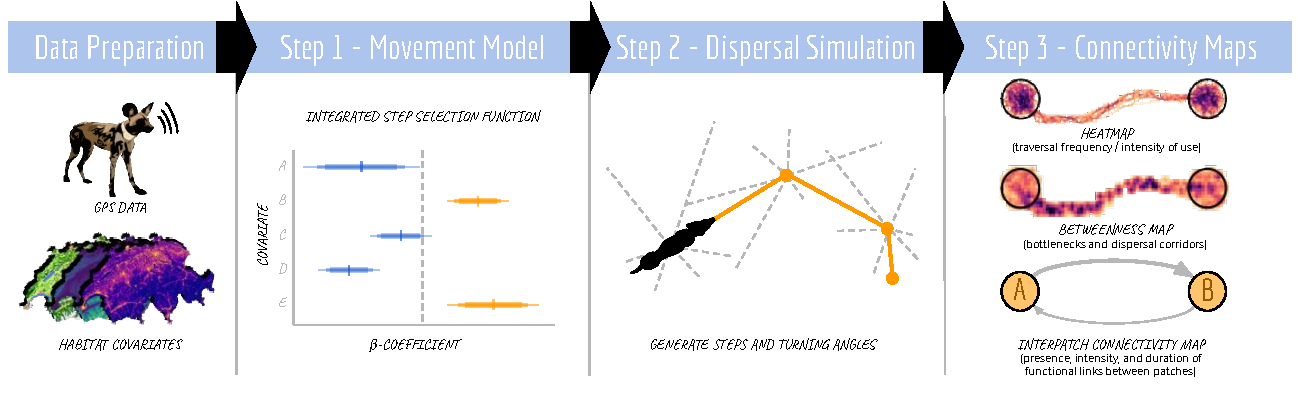
\includegraphics[width = \textwidth]{99_GraphicalAbstract2.pdf}
    \caption{Flowchart of the simulation-based connectivity analysis as proposed
    in this article. First, GPS data and habitat covariates have to be
    collected. The combined data is then analyzed in an integrated step
    selection model, which enables the parametrization of the focal species'
    habitat and movement kernels and results in a mechanistic movement model.
    The parametrized model is then treated as an individual-based movement model
    and used to simulate dispersal trajectories. Ultimately, simulated
    trajectories serve to produce a set of maps that are pertinent to landscape
    connectivity. This includes a heatmap, indicating the traversal frequency
    across each spatial unit of the study area, a betweenness map, highlighting
    movement corridors and bottlenecks, and, finally, an inter-patch
    connectivity map, where the frequency of connections and their average
    duration can be depicted.}
    \label{GraphicalAbstract}
  \end{center}
\end{figure}

% Case Study
\subsection{Case Study}
In this study, we illustrate the proposed three-step workflow
(\Cref{GraphicalAbstract}) to assess landscape connectivity for African wild
dogs within the Kavango-Zambezi Transfrontier Conservation Area (KAZA-TFCA), the
world's largest transboundary conservation area. To this end, we use GPS
movement data of 16 dispersing wild dogs originating from a free-ranging
population in northern Botswana to parametrize a mechanstic movement model,
which we then employed to simulate 80,000 dispersal trajectories across the
landscape of the KAZA-TFCA. We anticipated that simulations based on our
three-step workflow would overcome several of the above highlighted conceptual
shortcomings of traditional connectivity models and provide a more comprehensive
view of landscape connectivity.

\section{Methods}
\subsection{Study Area}
The study area centered at -17\degree 13'9''S, 23\degree 56'4''E
(\Cref{StudyArea}a) is located in southern Africa (\Cref{StudyArea}a) and spans
more than 1.3 Mio. km\textsuperscript{2}, encompassing the entire KAZA-TFCA
(\Cref{StudyArea}b). The KAZA-TFCA comprises parts of Angola, Botswana, Namibia,
Zimbabwe, and Zambia and hosts diverse landscapes; ranging from savannah to
grassland and from dry to moist woodland habitats. In its center lies the
Okavango Delta, a dominant hydrogeographical feature and the world's largest
flood-pulsing inland delta. Although large portions of the KAZA-TFCA are part of
designated national parks and other protected areas, considerable human
influence from roads, agricultural sites, and settlements remains.

\begin{figure}[h]
  \begin{center}
    \begin{tikzpicture}
        \node[anchor=south west,inner sep=0] (image) at (0,0,0) {
        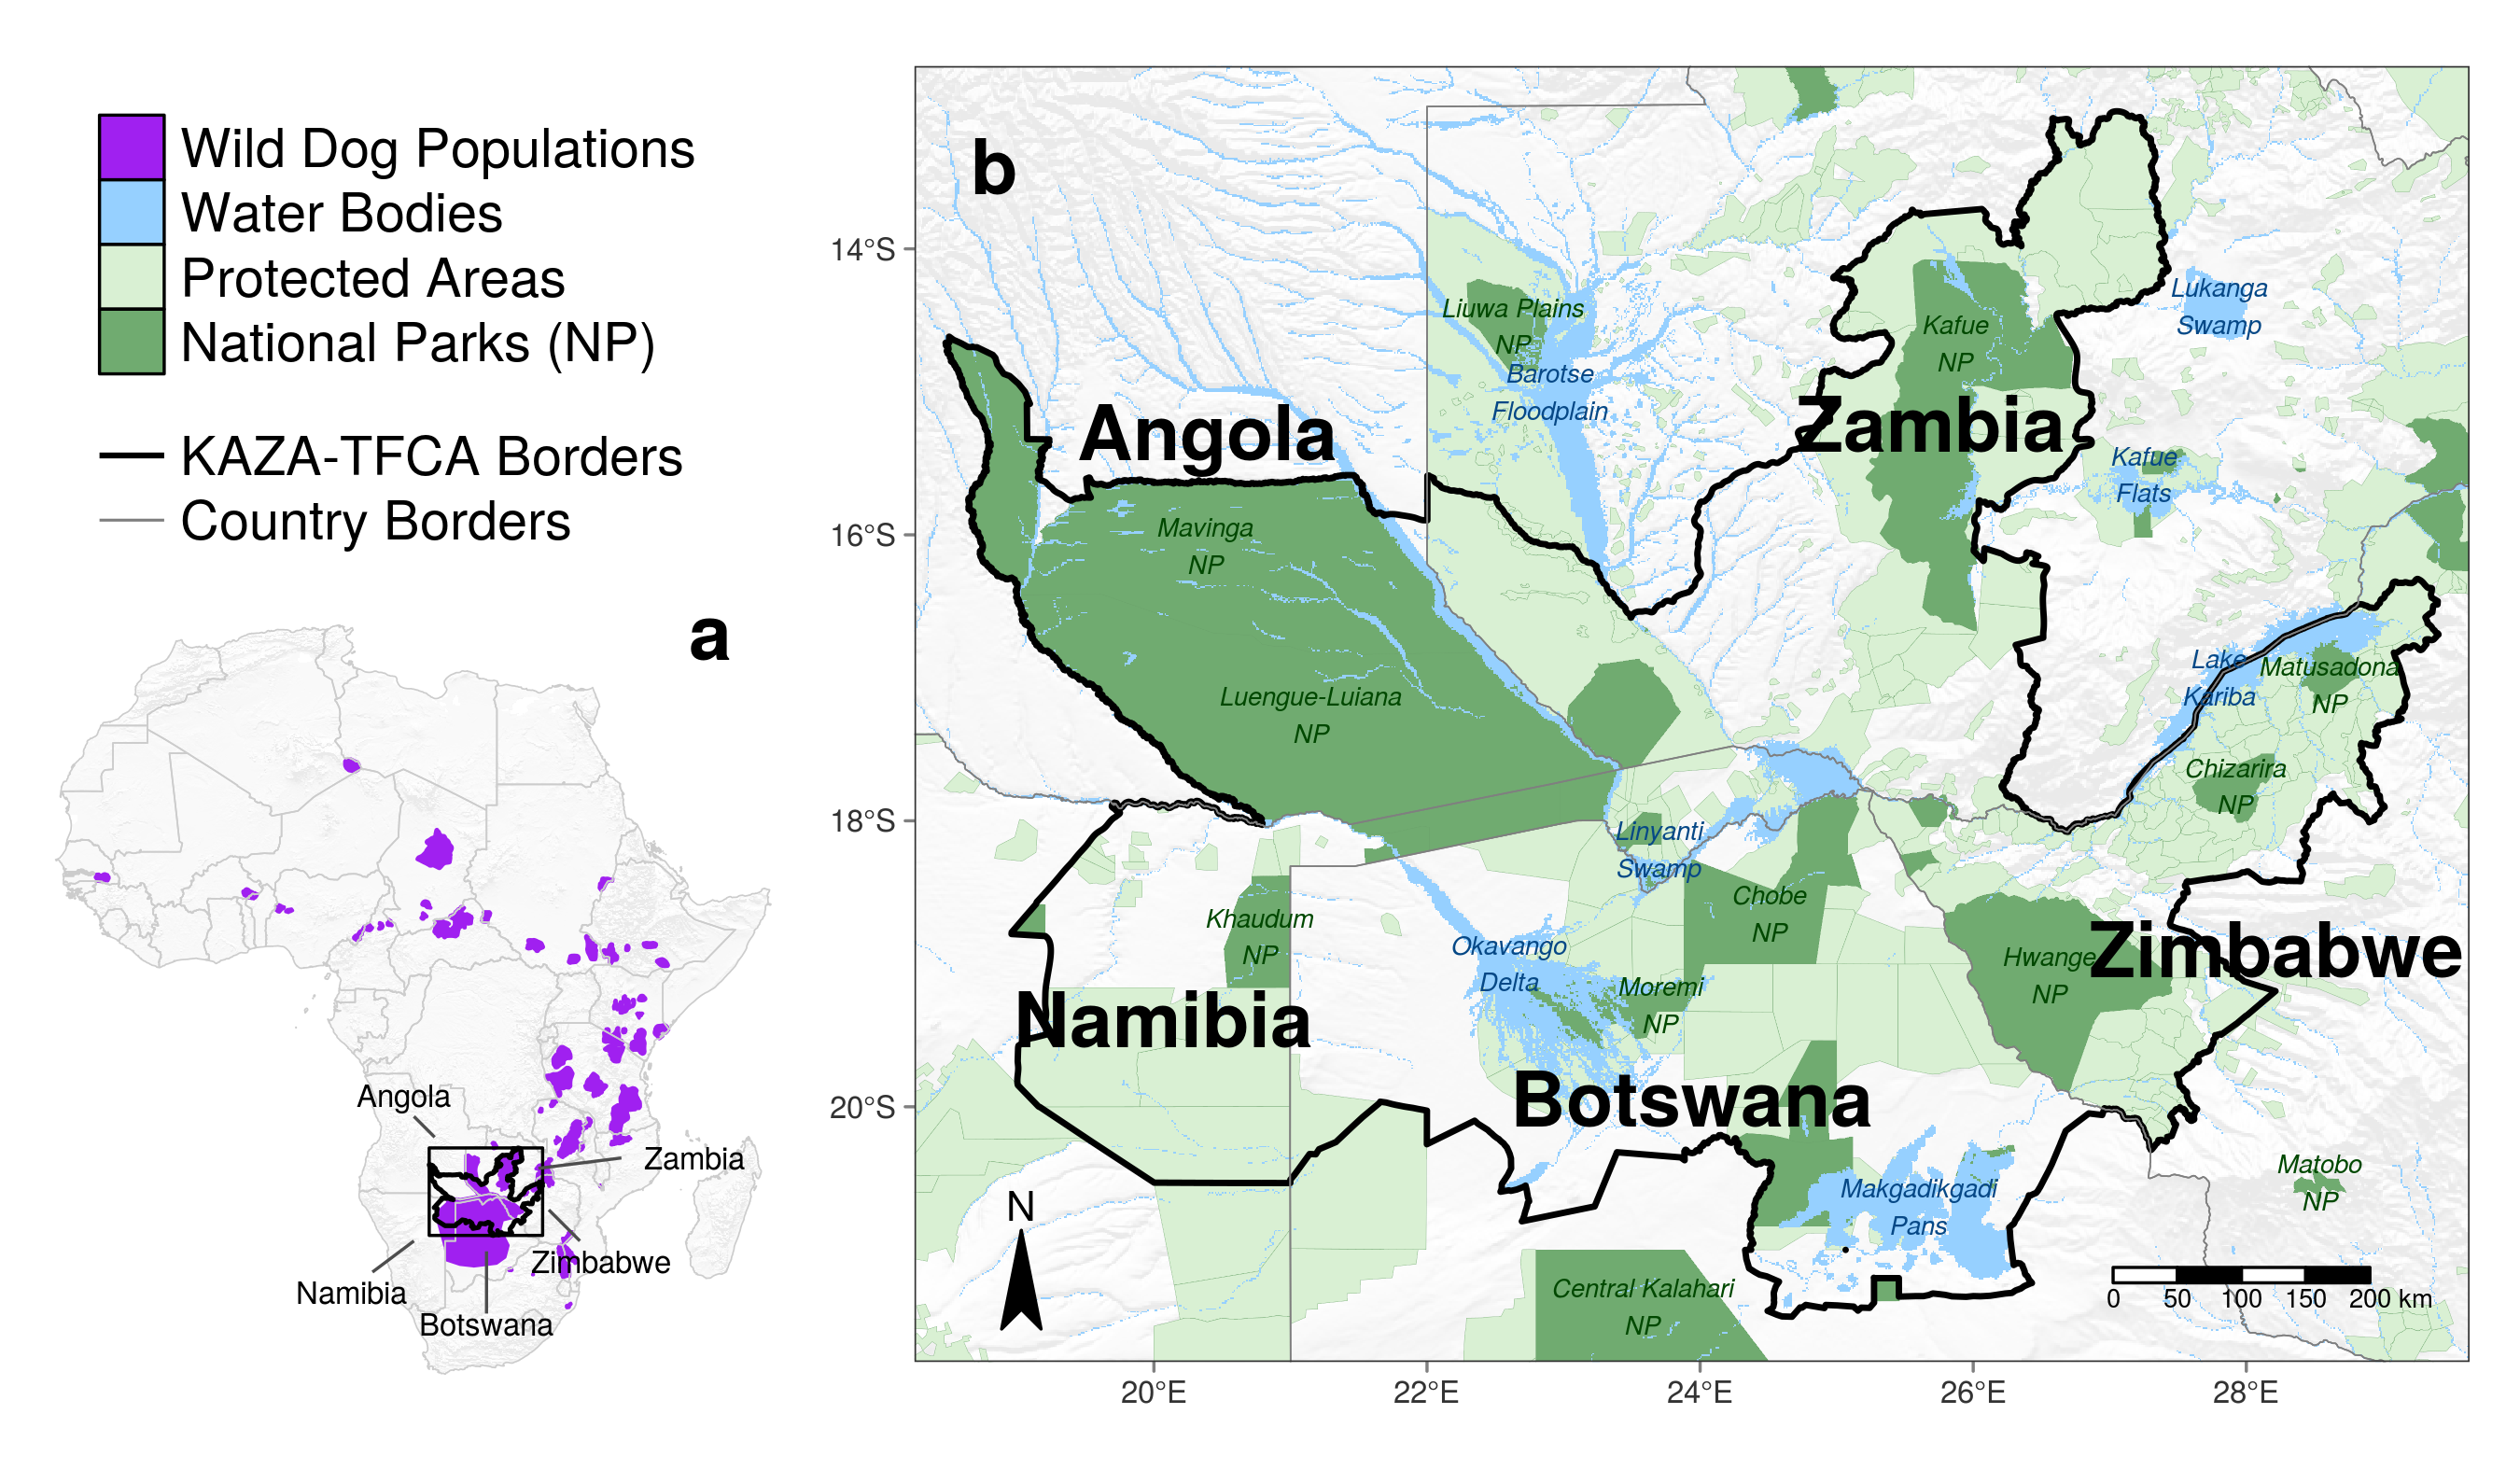
\includegraphics[width=\textwidth]{99_StudyArea.png}
        };
        \begin{scope}[x={(image.south east)},y={(image.north west)}]
            % % next four lines will help you to locate the point needed by forming a grid.
            % % comment these four lines in the final picture.
            % \draw[help lines,xstep=.1,ystep=.1] (0,0) grid (1,1);
            % \draw[help lines,xstep=.05,ystep=.05] (0,0) grid (1,1);
            % \foreach \x in {0,1,...,9} { \node [anchor=north] at (\x/10,0) {0.\x}; }
            % \foreach \y in {0,1,...,9} { \node [anchor=east] at (0,\y/10) {0.\y};}
            % % upto here
            \draw[densely dotted, blue] (0.169, 0.222) -- (0.364, 0.955);
            \draw[densely dotted, blue] (0.169, 0.157) -- (0.364, 0.074);
        \end{scope}
    \end{tikzpicture}
    \caption{Illustration of the study area located in southern Africa. (a) The
    study area was confined by a bounding box spanning the entire KAZA-TFCA and
    comprised parts of Angola, Namibia, Botswana, Zimbabwe, and Zambia. (b)
    The KAZA-TFCA represents the world's largest terrestrial conservation area
    and covers a total of 520'000 km\textsuperscript{2}. Its main purpose is to
    re-establish connectivity between already-existing national parks (dark
    green) and other protected areas (light green).}
    \label{StudyArea}
  \end{center}
\end{figure}

\subsection{Data Collection and Preparation}
\subsubsection{GPS Data}
We collected GPS movement data on 16 dispersing wild dogs (7 females and 9
males) between 2011 and 2019 from a free-ranging population in northern Botswana
(details on the data collection can be found in \cite{Cozzi.2020} and
\cite{Hofmann.2021}). Because behavior during dispersal is more pertinent to
landscape connectivity than behavior during residence \citep{Elliot.2014,
Abrahms.2017}, we discarded data collected when individauls were resident. We
determined the exact timing of emigration and settlement using direct field
observations and through visual inspection of the net squared displacement (NSD)
metric. NSD measures the squared Euclidean distance of a GPS relocation to a
reference point \citep{Borger.2012}, which we set to the center of each
dispersers' natal home range. Thus, dispersal was deemed to have started once an
individual left its natal home range and ended once the NSD metric ramined
constant, indicating settlement. During dispersal, GPS collars recorded a fix
every 4 hours and they regularly transmitted data over the Iridium satellite
system. To ensure regular timespans between fixes, we removed any fix that was
not obtained on the aspired 4-hourly schedule (\( \pm \) 15 minutes). We then
converted the remaining fixes (n = 4'169) into steps, where each step
represented the straight-line movement between two consecutive GPS relocations
\citep{Turchin.1998}.

\subsubsection{Habitat Covariates}
We represented the physical landscape in our study area by the habitat
covariates \textit{water-cover, distance-to-water, woodland-cover,
shrub/grassland-cover, and human-influence}. To reflect the seasonality of water
in the study area, we obtained weekly updated layers for water-cover and
corresponding layers for distance-to-water from MODIS satellite imagery using a
remote sensing algorithm \citealp{Wolski.2017, Hofmann.2021} that is implemented
in the \textsf{floodmapr} package which is available on GitHub
(\url{https://github.com/DavidDHofmann/floodmapr}). For each step, we thus used
the temporally associated water layers, reflecting prevailing conditions at the
time when the step was realized. To ensure a consistent resolution across
habitat covariates, we coarsened or interpolated all layers to a resolution of
250 m x 250 m. A more detailed description of how we prepared each habitat
covariate is provided in \cite{Hofmann.2021}.

Besides habitat covariates, we computed movement metrics that we used as
movement covariates in our ISSF analysis \citep{Avgar.2016, Fieberg.2021}.
Movement metrics were calculated for each step and included the step length
(\textsf{sl}), its natural logarithm (\textsf{log(sl)}), and the cosine of the
relative turning angle (\textsf{cos(ta)}).  Moreover, we created the binary
variable \textsf{LowActivity} indicating whether a step was realized during
periods of low wild dog activity (09:00 to 17:00 local time) or high wild dog
activity (17:00 to 09:00 local time, \citealp{Cozzi.2012}). We performed all
data preparations, spatial computations, and statistical analysis in R, version
3.6.6 \citep{R.2020}. Some helper functions were written in {\tt C++} and
imported into {\tt R} using the {\tt Rcpp} package \citep{Eddelbuettel.2011,
Eddelbuettel.2013}. We provide annotated R-codes to reproduce the three-step
workflow using simulated data through GitHub
(\url{https://github.com/DavidDHofmann/DispersalSimulation}). In addition, codes
for the African wild dog case study are available through an online repository.

\subsection{Step 1 - Movement Model}
We used ISSFs to parametrize a mechanistic movement model for dispersing wild
dogs \citep{Avgar.2016}. More specifically, we paired each realized step with 24
random steps, so that a realized step plus its 24 random steps formed a stratum
that received a unique identifier. As suggested by \cite{Avgar.2016}, we
generated random steps by sampling random turning angles from a uniform
distribution (\(-\pi, +\pi\))) (which is equivalent to a von Mises distribution
with concentration parameter \(\kappa = 0\)) and step lengths from a gamma
distribution that was fitted to realized steps (scale \(\theta\) = 6'308 and
shape \(k\) = 0.37)). Along each step, we extracted and averaged values from the
habitat covariate layers using the {\tt velox} package \citep{Hunziker.2021} and
calculated the movement metrics \textsf{sl}, \textsf{log(sl)}, and
\textsf{cos(ta)} for each realized and random step. To facilitate model
convergence, we standardized all continuous covariates to a mean of zero and a
standard deviation of one. Since correlation among covariates was low (\(|r| <
0.6\); \citealp{Latham.2011}), we retained all of them for modeling.

To contrast realized steps (scored 1) and random steps (scored 0), we assumed
that animals assigned a selection score \(w(x)\) of the exponential form to each
step \citep{Fortin.2005}. \(w(x)\) depended on the step's associated covariates
(\(x_1, x_2, ..., x_n\)) and on the animal's preferences (i.e. relative
selection strengths; \citealp{Avgar.2017}) towards these covariates (\(\beta_1,
\beta_2, ..., \beta_n\)):

\begin{equation}
\label{EQ1}
  w(x) = exp(\beta_1 x_1 + \beta_2 x_2 + ... + \beta_n x_n)
\end{equation}

The probability of a step being realized was then contingent on the step's
selection score, as well as on the selection scores of all other step in the
same stratum:

\begin{equation}
\label{EQ2}
  P(Y_{i} = 1 | Y_{1} + Y_{2} + ... + Y_{i} = 1) =
  \frac{w(x_{i})}{w(x_{1}) + w(x_{2}) + ... + w(x_{i})}
\end{equation}

\noindent To estimate preferences (i.e. the \(\beta\)-coefficients), we used
mixed effects conditional logistic regression analysis \citep{Muff.2020} that we
implemented using the r-package {\tt glmmTMB} \citep{Brooks.2017}. To capitalize
on the poisson trick introduced by \cite{Muff.2020}, we defined random
intercepts for each stratum and fixed the intercept variance to an arbitraty
high value of \(10 ** 6\). We also used disperser identity to model random
slopes for all covariates.

The covariate structure of the movement model was based on a habitat selection
model that we previously developed (hereafter referred to as based model,
\citealp{Hofmann.2021}). In the base model, no interactions among habitat
covariates and movement covariates were considered. Hence, we expanded the base
model and allowed for interactions between all movement covariates and habitat
covariates, thus reflecting that movement behavior may depend on habitat
conditions (details in Appendix AX). To assess the most parsimonious movement
model among model candidates, we ran stepwise forward model selection based on
Akaike's Information Criterion (AIC, \citealp{Burnham.2002}). Finally, we
validated the predictive power of the most parsimonious model using k-fold
cross-validation for case-control studies as desribed in \cite{Fortin.2009}. In
brief, this validation proofs a significant prediction in case the Spearman rank
correlation of predicted step ranks and associated frequencies under the
movement model is significantly stronger than under random preferences (details
in Appendix AX).

\subsection{Step 2 - Dispersal Simulation}
We used the most parsimonious movement model to simulate individual disperseral
trajectories within the study area. The simulation of a dispersal trajectory
resembled an ``inverted''  ISSF and was set up as follows. (1) We defined a
random source point and assumed a random initial orientation of the animal. (2)
Starting from the source point, we generated 25 random steps by sampling turning
angles from a uniform distribution (\(-\pi, +\pi\)) and step lengths from our
fitted gamma distribution. Like in the empirical data, each random step
represented the straight line movement possible within 4 hours. To prevent
unreasonably large steps, we restricted sampled step lengths to a maximum of 35
km (i.e. the farthest dispersal distance traveled within 4 hours in our data).
(3) Along each random step, we extracted and averaged values from the respective
habitat covariate layers and calculated movement covariates. To ensure
compatible scales with the fitted movement model, we standardized extracted
values using the mean and standard deviation from the empirical data. (4) We
applied the parametrized movement model to predict the selection score \(w(x)\)
for each step and we translated predicted scores into probabilities using
\ref{EQ2}. (5) We used predicted probabilities to sample one of the random steps
and determined the animal's new position. We repeated steps (2) to (5) until
2,000 steps (i.e. 400 consecutive dispersal days) were realized.\todo{Since we did not explain the 8-hourly gaps, this might be confusing}

To mitigate edge effects and to deal with random steps leaving the study area,
we followed \cite{Koen.2010} and artificially expanded all covariate layers by
a 100 km wide buffer zone. Within the buffer zone, we randomized covariate
values by resampling values from the original covariate layers. Through this
buffer zone, simulated dispersers were able to leave and re-enter the main study
area. In cases where proposed random steps transgressed the outer border of this
buffer zone, we resampled transgressing steps until they fully lied within the
buffer zone, forcing individuals to remain within the expanded study area.

For the simulation, we distributed 80,000 unique source points within the study
area. Of these, 50,000 were random locations inside protected areas that were
larger than the average home range size of wild dogs (i.e. \(>\) 700
km\textsuperscript{2}; \citealp{Pomilia.2015}), while the remaining 30,000
source points were placed randomly inside the buffer zone, mimicing potential
immigration into the study area (Figure S1). Due to the random distribution of
source points, the number of source points per km\textsuperscript{2} in selected
areas was approximately equal.

To ensure reliable connectivity estimates, we determined the number of simulated
dispersal trajectories required for connectivity to reach a  ``steady state''
across the entire study area. For this purpose, we distributed 1,000 rectangular
``checkpoints'', each with an extent of 5 km x 5 km at random coordinates within
the study area (excluding the buffer). We then determined the relative frequency
at which each checkpoint was traversed by simulated dispersers (hereafter
referred to as relative traversal frequency) as we gradually increased the
number of simulated trajectories from 1 to 50,000. To assess variability in the
relative traversal frequency, we repeatedly subsampled 100 times from all 50'000
dispersal trajectories and computed the mean traversal frequency across
replicates, as well as its 95\% confidence-interval for each checkpoint. We
considered connectivity to have reached a steady state once the width of the
prediction-interval dropped below a value of 0.01 for all checkpoints.

\subsection{Step 3 - Connectivity Maps}
\subsubsection{Heatmap}
To identify dispersal hotspots within the study area, we created a heatmap
indicating the absolute frequency at which each raster-cell was traversed by
simulated dispersers (e.g. \citealp{Peer.2008, Hauenstein.2019, Zeller.2020}).
That is, we rasterized all simulated trajectories onto a raster with 250 m x 250
m resolution and tallied them into a single map. If the same trajectory crossed
a raster-cell twice, we only counted it once, thereby mitigating biases from
individuals that were trapped and moved in circles. To achieve high performance
rasterization, we used the R-package {\tt terra} \citep{Hijmans.2021b}.

\subsubsection{Betweenness Map}
To pinpoint discrete movement corridors and bottlenecks, we converted simulated
trajectories into a network and calculated betweenness scores for all
raster-cells in the study area \citep{BastilleRousseau.2018}. Betweenness
measures how often a specific network-node (i.e. raster-cell) lies on a shortest
path between any other pair of nodes and is therefore pertinent to connectivity
\citep{BastilleRousseau.2018}. To transform simulated trajectories into a
network, we followed \citep{BastilleRousseau.2018} and overlaid the study area
(including the buffer) with a 5 km x 5 km raster, where the center of each
raster-cell served as node in the final network. To identify edges (i.e.
connections) between the nodes, we used the simulated trajectories and
determined all transitions occurring from one node to another, as well as the
frequency at which those transitions occurred. This resulted in an edge-list
that we translated into a weighted network using the r-package {\tt igraph}
\citep{Gabor.2006}. The weight of each edge was determined by the frequency of
transitions, yet because {\tt igraph} handles edge weights (\(\omega\)) as
costs, we had to invert the traversal-frequency thorugh each raster-cell by
applying \(\omega = \frac{mean(Traversal Frequency)}{Traversal Frequency_i}\).
Consequently, edges that were traversed frequently were assigned small weights
and vice versa. Finally, we used the weighted network to calculate betweenness
scores at all network nodes.

\subsubsection{Inter-Patch Connectivity Map}
To examine the presence and intensity of functional links (i.e. connections)
between specific patches inside the KAZA-TFCA, we calculated inter-patch
connectivity between national parks. The decision to only consider national
parks as our  ``patches'' was purely out of simplicity and does not imply that
connections between other protected areas are impossible. To quantify
inter-patch connectivity, we computed the relative frequency at which dispersers
originating from one national park successfully moved into another national
park. We considered movements successful if the individuals' dispersal
trajectory intersected with the target national park at least once. We also
recorded the number of steps required to reach the first intersection with the
respective national park, allowing us to compute the average dispersal durations
from one park to another. In summary, we determined \textit{if} and \textit{how
often} dispersers moved between certain national parks, as well as \textit{how
long} individuals had to move to make these connections.

\section{Results}
\subsection{Movement Model}
The most parsimonious movement model consisted of movement covariates, habitat
covariates and several of their interactions, suggesting that movement behavior
during dispersal depends on habitat conditions (\Cref{MovementModel}, Table S1
and Table S2). Although multiple models received an AIC weight > 0 (Table S1),
we only considered results from the most parsimonious model for simplicity. This
decision only marginally influenced subsequent steps as all models with positive
AIC weights contained similar covarites (Table S1). Aids for interpreting main
effects and interactions are provided in Figure S2. Under average conditions,
dispersing wild dogs avoided moving through water, woodlands, and areas
dominated by humans, but preferred shrublands or grasslands
(\Cref{MovementModel}). Dispersers realized shorter steps (indicating slower
movements) in areas covered by water or woodland, while realizing larger steps
in areas dominated by shrubs or grass. Moreover, dispersing wild dogs moved
faster during twilight and at night (i.e. between 17:00 and 09:00 o'clock) than
during the rest of the day. Although dispersers showed a preference for
directional movements, especially when moving quickly, they did less so in
proximity to humans or water, resulting in more tortuous movements in such
areas.

% When all other covariates held constant at their means, the habitat kernel
% reveals that dispersing wild dogs avoid water but prefer its proximity, that
% dispersers avoid areas that are covered by woodlands, yet prefer regions covered
% by shrublands or grasslands, and that dispersers avoid movement through
% landscapes that are dominated by humans. All of these effects are strong and
% significant, except for the effect of \textsf{distance to water}, which is
% insignificant on the 5\% significance level.
%
% With regards to the movement kernel, the positive estimate for \textsf{cos(ta)}
% indicates that dispersers move with directional persistence, unlike what was
% proposed by the uniform turning angle distribution. This preference is
% particularly pronounced when dispersers realize large steps (i.e. move quickly),
% as indicated by the positive estimates for \textsf{cos(ta):sl} and
% \textsf{cos(ta):log(sl)}. Finally, the negative estimate for the interaction
% \textsf{sl:LowActivity} reveals that wild dogs realize shorter steps (i.e. move
% slower) between 09:00 and 17:00 o'clock than during the rest of the day. Aside
% from the interaction \textsf{sl:LowActivity}, which has a very strong effect,
% effects are moderate strength yet significant on the 5\% significance level;
% only the interaction \textsf{cos(ta):sl} appears as insignificant on the 5\%
% significance level.
%
% Finally, several significant interactions between movement and habitat
% covariates suggest that movement behavior is contingent on habitat conditions.
% For example, there's strong evidence that dispersers realize shorter steps in
% areas covered by water or in forested areas. Furthermore, it appears that
% dispersers realize larger steps in areas that are dominated by shrubs/grassland,
% but shorter steps in areas that are distant to water. Finally, it seems that the
% preference for directional persistence is less pronounced when dispersers cross
% human-dominated landscapes, yet more pronounced at great distance from water.
% Nevertheless, some of these effects are only weakly significant and exhibit
% small effect sizes.

The k-fold cross-validation of the movement model showed that the final model
substantially outperforms a random guess , suggesting reliable predictions
(confidence intervals of \(\bar{r}_{s, realized}\) and \(\bar{r}_{s, random}\)
do not overlap). Moreover, the model correctly assigns high selection scores to
realized steps (\Cref{MovementModel}b), indicating a good fit between
predictions and observations. Compared to the base model (\(\bar{r}_{s,
realized} = -0.55; 95\%-CI = [-0.57, -0.52]\); \citealp{Hofmann.2021}), the
inclusion of several interactions between movement and habitat covariates
significantly improved model performance (\(\bar{r}_{s, realized} = -0.65;
95\%-CI = [-0.67, -0.64]\).

\begin{figure}
  \begin{center}
    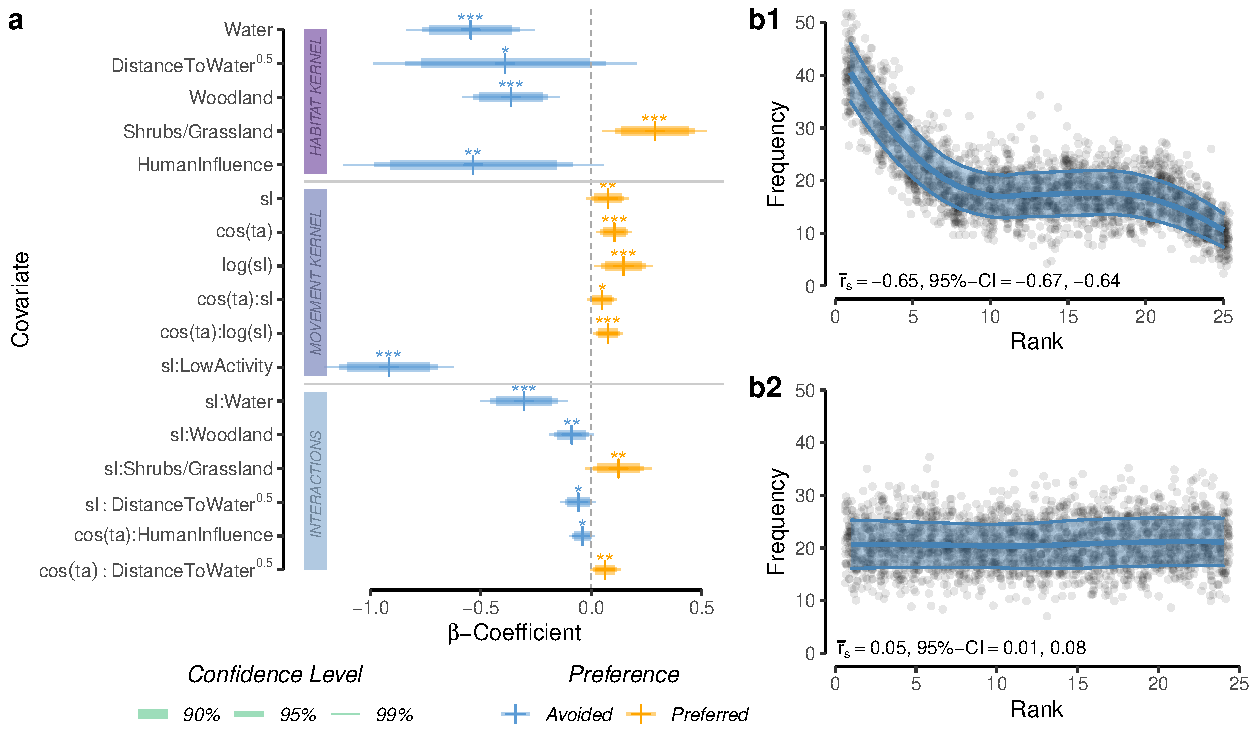
\includegraphics[width=\textwidth]{99_MovementModel}
    \caption{(a) Most parsimonious movement model for dispersing wild dogs. The
    model comprises a habitat kernel, a movement kernel, as well as their
    interactions. The horizontal line segments delineate the 90\%, 95\%, and
    99\% confidence-intervals for the respective \(\beta\)-coefficients.
    Significance codes: * \(p < 0.10\), ** \(p < 0.05\), *** \(p < 0.01\). (b)
    Results from the k-fold cross validation procedure. The upper plot shows
    rank frequencies of realized steps according to model predictions with known
    preferences, whereas the lower plot shows rank frequencies of realized steps
    when assuming random preferences. The blue ribbon shows the prediction
    interval around a loess smoothing regression that we fitted to ease the
    interpretation of the plots. The significant correlation between rank and
    associated frequency in (b1) highlights that the most parsimonious model
    successfully outperforms a random guess (b2) and assigns comparably high
    selection scores to realized steps.}
    \label{MovementModel}
  \end{center}
\end{figure}

\subsection{Dispersal Simulation}
Our dispersal simulations based on the most parsimonious movement model proved
useful for assessing landscape connectivity. Of the 50,000 simulated dispersers
initiated within the main study area, only 4.5\% were eventually repelled by a
map boundary, suggesting minimal biases due to boundary effects. Moreover, our
examination of relative traversal frequencies across all checkpoints suggested
that connectivity reached a steady state after 10,500 simulated dispersal
trajectories (Figure S3). Although variability in relative traversal frequencies
kept decreasing as we increased the number of simulated dispersers, the marginal
benefit of additional trajectories diminished quickly (Figure S3).

\subsection{Heatmap}
The heatmap (\Cref{Heatmap}), which resulted from the summation of all simulated
dispersal trajectories, showed that several extensive regions within the
KAZA-TFCA were frequently traversed by dispersing wild dogs (mean traversal
frequency = 166, IQR = 274, Figure S6a), while areas beyond the KAZA-TFCA
boundary were rarely visited (mean traversal frequency = 61, IQR = 133, Figure
S6a). Most notably, the region in northern Botswana south of the Linyanti swamp
appeared as highly frequented dispersal hotspot (mean traversal frequency = 987,
IQR = 558). Nevertheless, the presence of extensive water bodies, such as the
Okavango Delta, the Makgadikgadi Pan, and the Linyanti swamp, restricted
dispersal movements and limited realized connectivity within the KAZA-TFCA.
Similarly, high human densities, roads, and agricultural activities in Zambia's
and Zimbabwe's part of the KAZA-TFCA limited dispersal movements. Outside the
KAZA-TFCA, the most heavily used regions included the areas inside the Central
Kalahari National Park in Botswana, the area south-west of the Khaudum National
Park in Namibia, and the area surrounding the Liuwa Plains National Park in
Zambia. Although the heatmap facilitated the identification of areas frequently
traversed by simulated dispersers, it seemed impractical to pinpoint dispersal
corridors.

\begin{figure}
  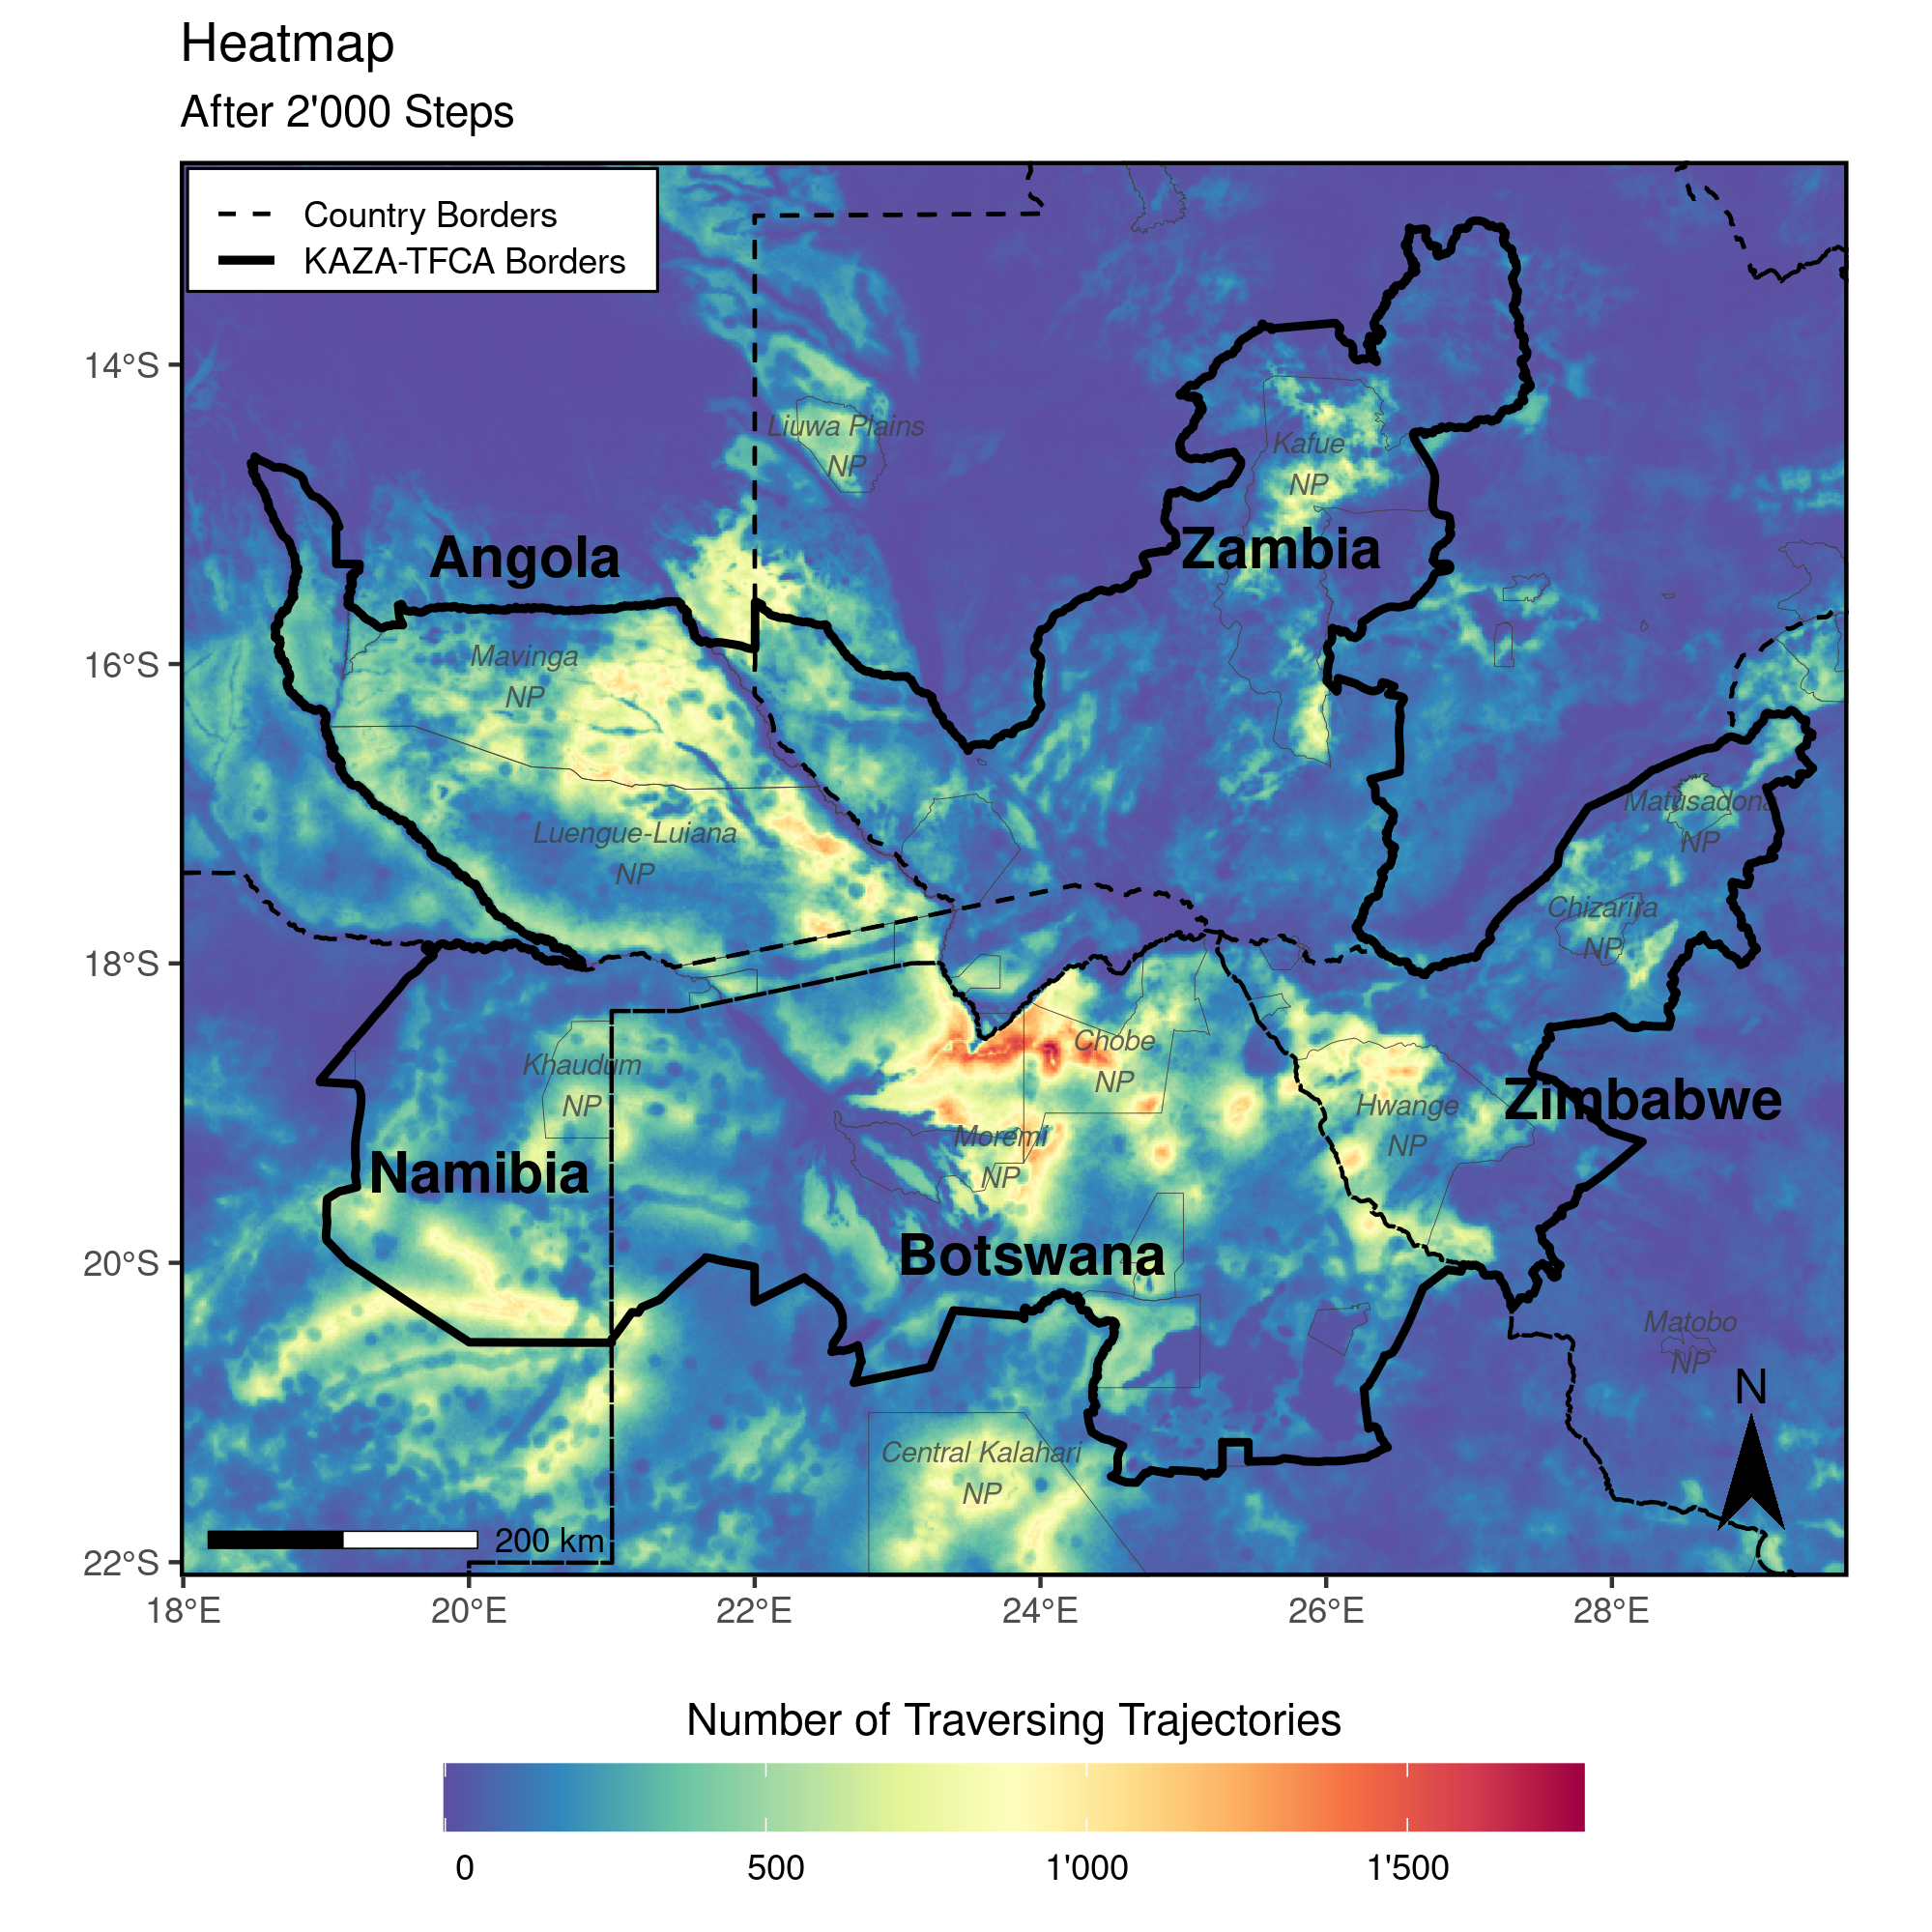
\includegraphics[width=\textwidth]{99_Heatmap.png}
  \caption{Heatmap showing traversal frequencies of 80'000 simulated dispersers
  moving 2'000 steps across the KAZA-TFCA. Simulations were based on an
  integrated step selection model that we fitted to the movement data of
  dispersing African wild dogs. To generate the heatmap, we rasterized and
  tallied all simulated trajectories. Consequently, the map highlights areas
  that are frequently traversed by virtual dispersers. For spatial reference we
  plotted a few selected national parks (dark gray). Additional heatmaps showing
  the traversal frequency when individuals move fewer than 2'000 steps are
  provided in Figure S4.}
  \label{Heatmap}
\end{figure}

\subsection{Betweenness}
The betweenness map (\Cref{Betweenness}) revealed distinct dispersal corridors
that run within the KAZA-TFCA . Again, the region in northern Botswana emerged
as wild dog dispersal hub that connected more remote regions in the study area.
Towards east, the extension of this corridor ran through Chobe National Park
into Hwange National Park. From there, a further extension connected to
Matusadona National Park in Zimbabwe. Northwest of the Linyanty ecosystem, a
major corridor expanded into Angola, where it splitted and finally traversed
over a long stretch of unprotected area into Zambia's Kafue National Park.
Several additional corridors with lower betweenness scores emerged, yet most of
them ran within the KAZA-TFCA boundaries (median betweenness inside KAZA-TFCA =
6947\(k\), IQR = 54311\(k\), Figure S6b). In general, there were few corridors
that directly linked the peripheral regions of the KAZA-TFCA and passed through
unprotected areas outside the KAZA-TFCA (mean betweenness outside KAZA =
2685\(k\), IQR = 9891\(k\), Figure S6b). Compared to the heatmap, the
betweenness map facilitated the identification of dispersal corridors between
habitat patches.

%  9 2000  Betweenness Inside KAZA-TFCA  6946817.   54311358.
% 10 2000  Betweenness Outside KAZA-TFCA 2685174.    9890504.

\begin{figure}
  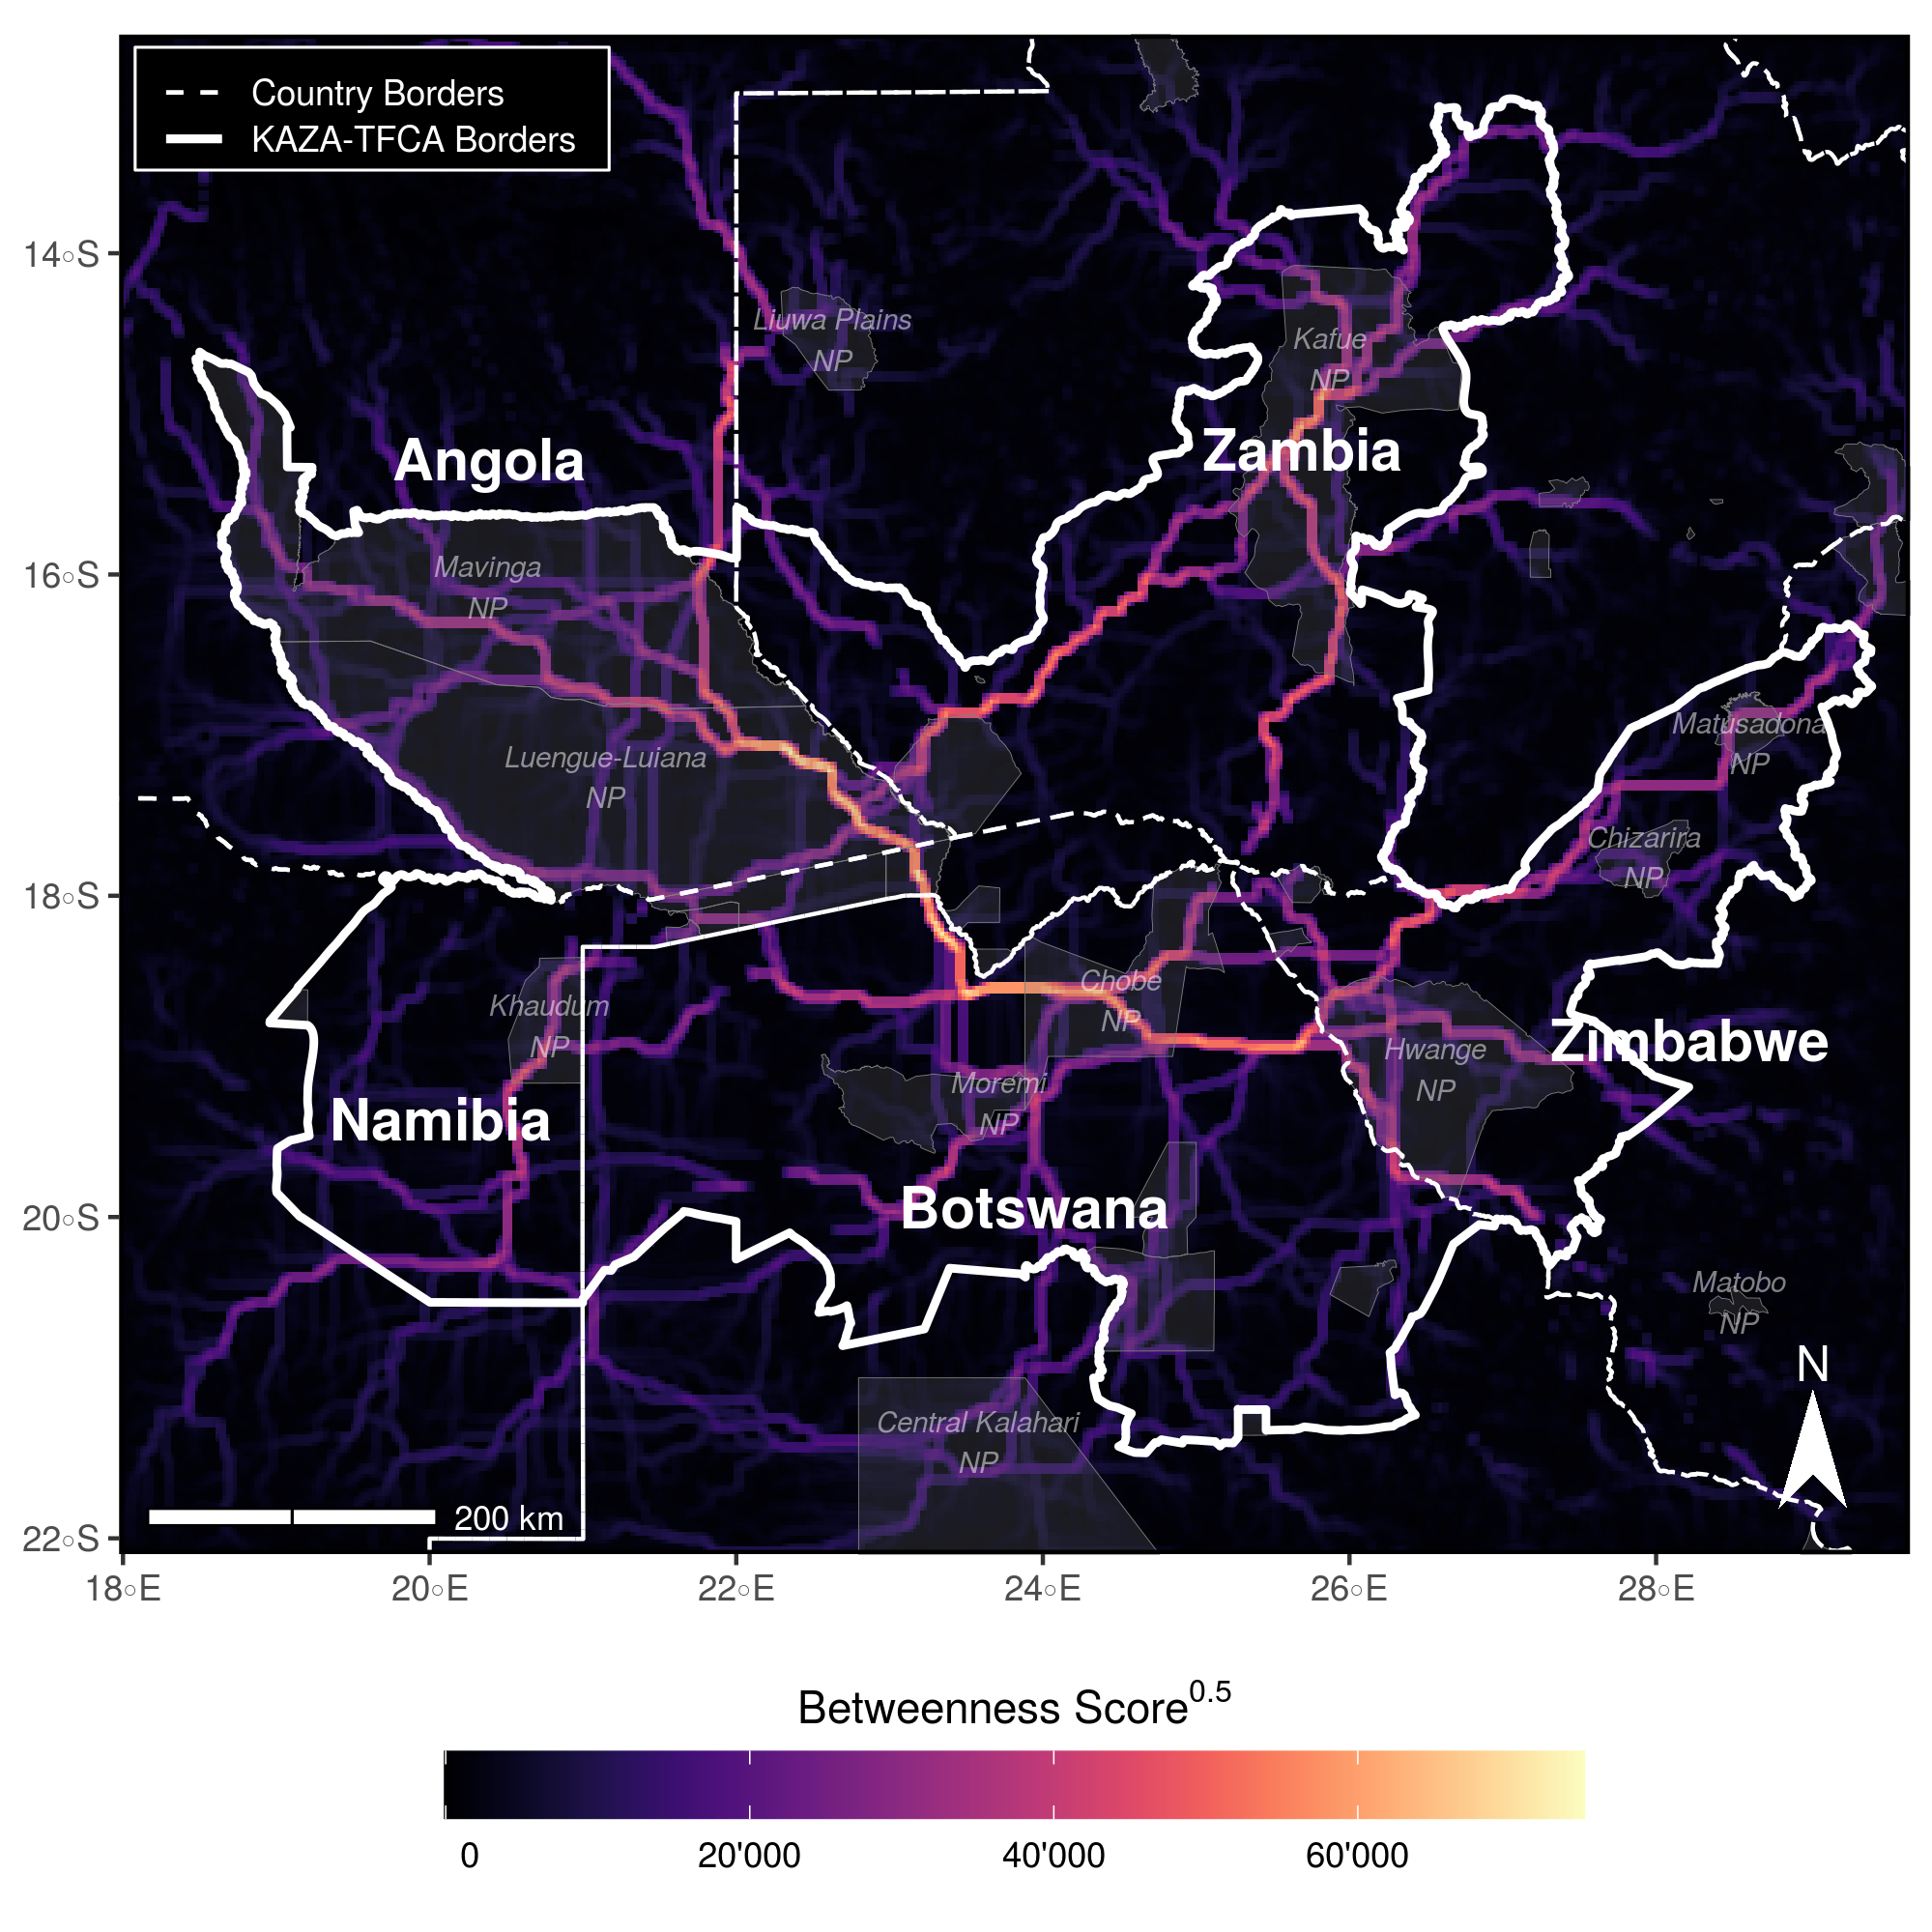
\includegraphics[width=\textwidth]{99_Betweenness.png}
  \caption{Map of betweenness scores, highlighting distinct dispersal corridors
  and potential bottlenecks across the extent of the KAZA-TFCA. A high
  betweenness score indicates that the respective area is exceptionally
  important for connecting different regions in the study area. In this sense
  the metric can be used to pinpoint discrete movement corridors
  \citep{BastilleRousseau.2018}. Note that we square-rooted betweenness scores
  to improve visibility of corridors with low scores. Additional betweenness
  maps showing betweenness scores when individuals move fewer than 2'000 steps
  are provided in Figure S4.}
  \label{Betweenness}
\end{figure}

\subsection{Inter-Patch Connectivity}
The map of inter-patch connectivity showed that the relative frequency at which
simulated dispersers moved from one national park to another varied, as did the
average dispersal duration required to make these connections
(\Cref{InterpatchConnectivity}). Overall, interpatch connectivity between
national parks in Angola, Namibia, and Botswana appeared to be high (mean
relative frequency = +- ) with short dispersal durations (mean duration = +-)


Results from the analysis of inter-patch connectivity are given in
\Cref{InterpatchConnectivity}, which shows all realized links by simulated
dispersers between national parks. The map furthermore indicates the relative
frequency at which dispersers originating from one national park successfully
reached another national park, as well as the average duration dispersers had to
move to realize those links. It is again worth pointing out that the figure is
only intended as an illustration, as for clarity we only considered inter-patch
connectivity between national parks (NPs), albeit plenty of links between other
protected areas exist. Overall, inter-patch connectivity between NPs in Angola,
Namibia, and Botswana appears to be high, with relatively short dispersal
durations between national parks. In contrast, we observe that connections from
the central region into the Kafue NP in Zambia require rather long dispersal
events and are rather infrequent. Similarly, relatively few connections lead
into Zimbabwe's Chizarira and Matusadona NP. In some cases, we also find
imbalances between ingoing and outgoing links, hinting at potential source-sink
dynamics that occur due to asymmetries in disperser's willingness to cross an
area, depending on the direction in which the area is traversed. For instance,
while a fair share of dispersers originating from the Chizaria NP in Zimbabwe
manages to move into the Hwange NP, there are comparably few dispersers that
succeed in the opposite direction.

% The map shows all realized links by simulated dispersers between national parks
% and indicates the average duration a disperser had to move to realize those
% links. For instance, 6.8 \% of the simulated dispersers originating from the
% Moremi National Park successfully reached the Chobe National Park and 4.2 \% the
% Hwange National Park in Zimbabwe. On average, dispersers moved for 623 steps
% before arriving at Chobe (SD = 520) and for 1'413 steps before arriving at
% Hwange (SD = 371). While the map only depicts connections between national
% parks, this does not imply that no connections to other protected areas exist
% and is the result of our simplifying assumptions above. Interestingly, while we
% identified a potential dispersal corridor between Angola's NPs and the Kafue NP
% in Zambia, \Cref{InterpatchConnectivity} suggests that this link is only
% rarely realized and requires very long dispersal events. In contrast, we find
% that dispersal between the Moremi NP and Chobe NP are relatively frequent and
% require fewer steps, which can be expected given that the areas are located
% close to each other.

\begin{figure}
  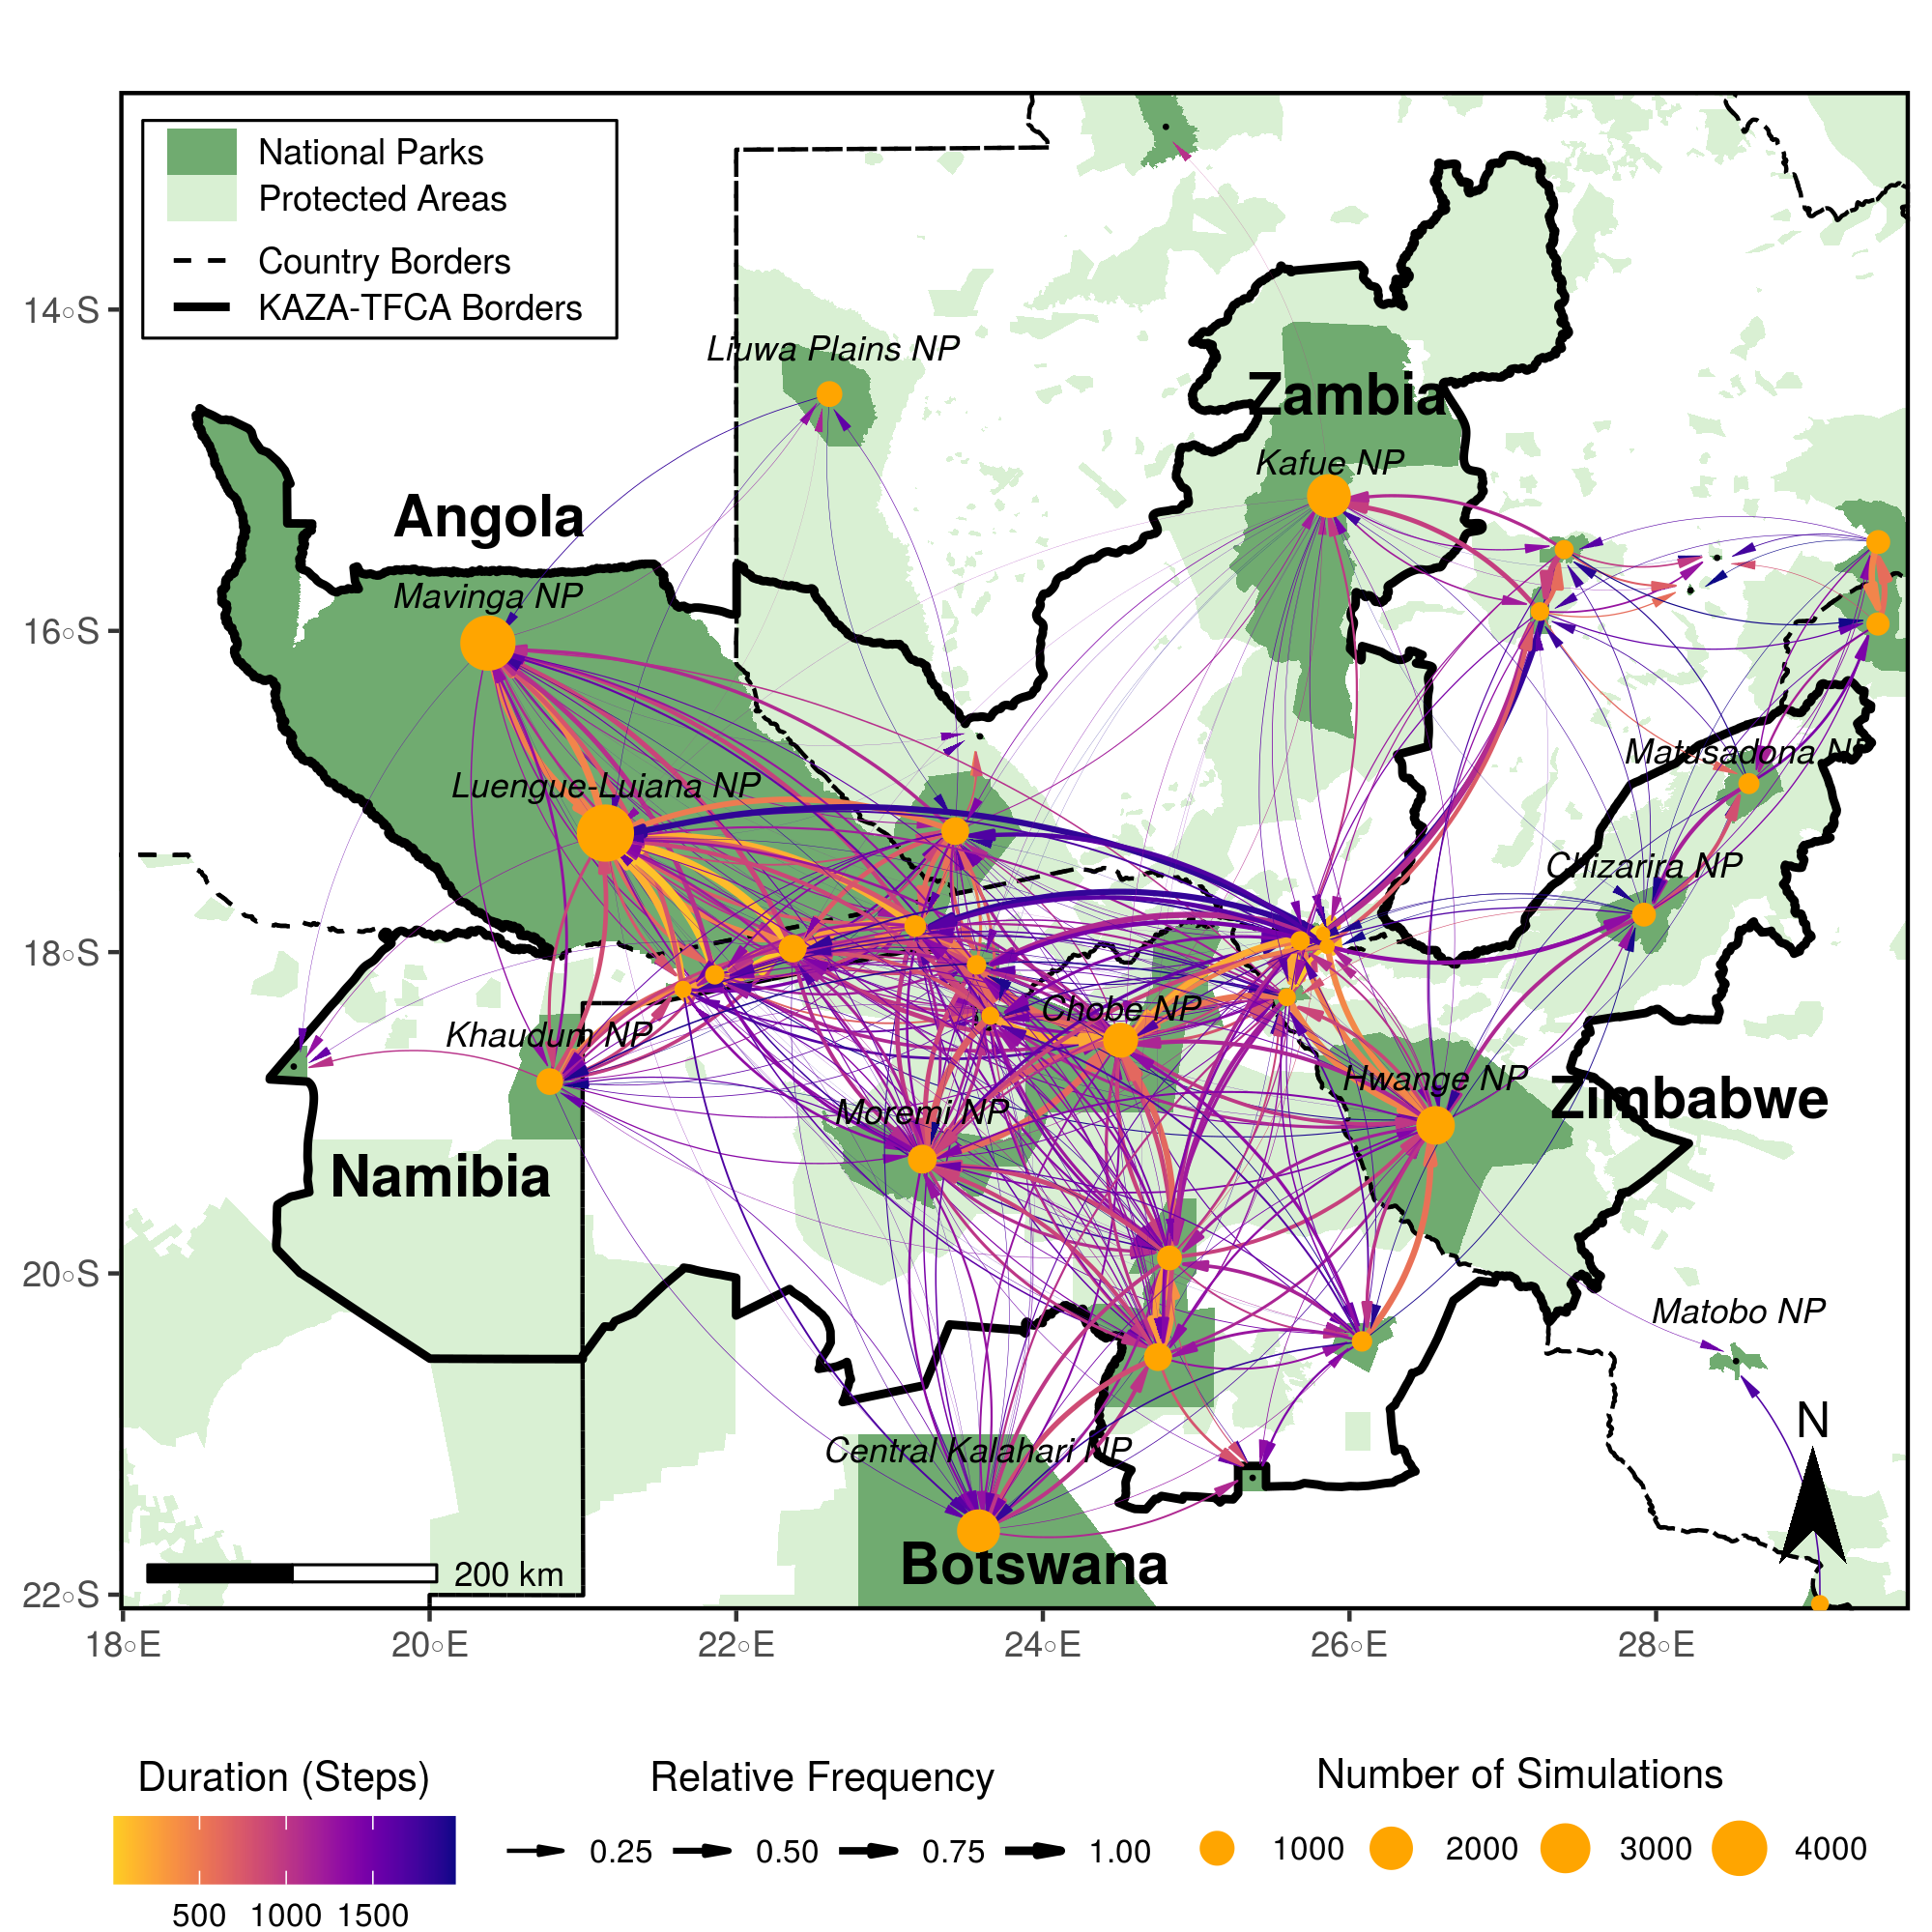
\includegraphics[width=\textwidth]{99_InterpatchConnectivity.png}
  \caption{Map of inter-patch connectivity, highlighting connections between
  national parks (dark green). Yellow bubbles represent the center of the
  different national parks and are sized in relation to the number of simulated
  dispersers originating from each park. Black dots represent national parks
  that were smaller than 700 km\textsuperscript{2} and therefore did not serve
  as source areas. Arrows between national parks illustrate between which
  national parks the simulated dispersers successfully moved and the color of
  each arrow shows the average number of steps (4-hourly movements) that were
  necessary to realize those connections. Additionally, the line thickness
  indicates the relative number of dispersers originating from a national park
  that realized those connections. Note that a similar network view could be
  adopted to investigate connectivity between other protected areas need not to
  be restricted to national parks.}
  \label{InterpatchConnectivity}
\end{figure}

\section{Discussion}

% Short Summary
\subsection{Short Summary}
We used ISSFs to analyse data of dispersing wild dogs and to parametrize a fully
mechanistic movement model describing how dispersers move through the available
landscape. We employed the parametrized model as an individual-based movement
model to simulate 80'000 dispersing wild dogs moving 2'000 steps across the
extent of the KAZA-TFCA, the world's largest transboundary conservation area.
Based on simulated dispersal trajectories, we derived three complementary maps,
each geared towards a better understanding of dispersal and landscape
connectivity. The set of maps included a heatmap, revealing frequently traversed
areas, a betweenness-map, delineating critical dispersal corridors, and a map of
inter-patch connectivity, indicating the presence or absence of functional links
between national parks as well as the average dispersal duration required to
realize those links. We thereby showcase that ISSFs offer a simple, yet powerful
framework to parametrize movement models and simulate dispersal to assess
landscape connectivity. Importantly, individual-based simulations from ISSFs
overcome several conceptual shortcomings inherent to more traditional
connectivity modeling techniques, such as LCPA and CT.

% Movement Model
\subsection{Movement Model}
Because our movement model of dispersing wild dogs comprised two interacting
kernels, it effectively rendered habitat and movement preferences of dispersers,
as well as how preferences depended on habitat conditions. Results from the
habitat kernel were largely in concert with previous studies that investigated
habitat selection by dispersing wild dogs \citep{DaviesMostert.2012,
Masenga.2016, Woodroffe.2019, Oneill.2020, Hofmann.2021}. However, by also
incorporating a movement kernel, we were able to model several additional
complexities inherent to dispersal. For instance, we could accommodate that
dispersers move with directional persistence \citep{Cozzi.2018, Hofmann.2021}
and exhibit step lengths that are correlated with turning angles
\citep{Morales.2004, Borger.2012} by including the appropriate interactions in
the movement model. While correlations between step lengths and turning angles
could also be rendered by sampling them from copula probability distributions
\citep{Hodel.2021a, Hodel.2021b}, the ISSF framework allowed us to directly
incorporate them in the movement model. In addition, by forming interactions
between habitat covariates and movement covariates, we could render potential
dependencies between movement and habitat preferences. For example, our final
model contained an interaction between water-cover and step length, showing that
dispersers realize shorter steps in areas covered by water. Likewise, we found
that dispersers move more tortuously across water bodies than over dryland,
which is clearly to be expected, given that wild dogs have to wade or swim when
traversing waterbodies. The ability of accompanying such effects in a single
model is one of the great strengths of ISSFs \citep{Avgar.2016, Fieberg.2021},
which is why we believe the method offers a suitable framework for simulating
movement and assessing connectivity.

\subsection{Simulation}
Our simulation of 80'000 dispersers moving 2'000 steps across the landscapes of
the KAZA-TFCA required five days of computation on a modern desktop machine.

On a machine with an octa-core AMD Ryzen 7 2700X processor (8 x 3.6 GHz, 16
logical cores) and 64 GB of RAM, a batch of 1'000 simulated dispersers moving
over 2'000 steps required 90 minutes to compute (\(\mu = 88.90\), \(\sigma =
1.87\)). Consequently, the simulation of all 80'000 dispersers (160 Mio. steps)
terminated after 120 hours (i.e. five days). Comparable simulations will be
substantially faster for smaller study areas and lower resolution covariates, as
the covariate extraction from large and high-resolution rasters was
computationally the most demanding task. Out of the 50'000 dispersers initiated
inside the main source area, only 4.5\% were eventually repelled by a map
boundary, suggesting that biases due to boundary effects should be minimal.

 The
long simulation time was primarily caused by the massive extent considered (ca.
1.8 Mio. km\textsuperscript{2} when including the buffer) and the large number
of dispersers simulated. Most connectivity studies are limited to much smaller
extents (e.g. \citealp{Kanagaraj.2013, Clark.2015, McClure.2016, Abrahms.2017,
Zeller.2020}) and will therefore achieve faster simulation times. We also
believe that fewer simulated dispersers will often suffice, as the relative
traversal frequency by simulated individuals through randomly placed checkpoints
in the study area converged already after 10'500 simulated individuals. However,
the required number of simulated individuals to achieve reliable estimates of
connectivity will vary depending on the structure of the landscape and the
dispersal ability of the focal species.

\subsection{Maps}
The heatmap generated from simulated dispersal trajectories highlighted that
numerous individuals traversed the Moremi NP and the Chobe NP in northern
Botswana. We previously uncovered the same area as potential dispersal hotspot
using least-cost methods \citep{Hofmann.2021}, yet it has been questioned
whether this was a consequence of the region being located in the center of the
study area and connections being enforced between predefined start and
endpoints. With the current simulations, connections were no longer enforced and
simulated individuals were able to leave the main study area. Nonetheless, a
majority of simulated individuals traversed the area in northern Botswana. This
suggests that the dispersal hotspot is not merely an artifact of the applied
method but truly results from landscape characteristics. The same region is also
pronounced on the betweenness map, implying that it facilitates the relocation
of individuals into more remote regions of the KAZA-TFCA. While this is an
example of an area where both the heatmap and the betweenness map attest great
importance, there are other instances where this is not true. For example, while
the area between the Lengue-Luiana NP in Angola and the Kafue NP in Zambia
receives a high betweenness-score, the heatmap shows that the area is only
rarely traversed by dispersers. Hence, despite the region's importance for
linking Angola's NPs to Zambia's NP, only few simulated dispersers actually used
the corridor. Conversely, we find that the Central Kalahari NP receives a low
betweenness score, despite being highly frequented by simulated dispersers.
Besides highlighting frequently traversed areas and dispersal corridors, we also
also consulted inter-patch connectivity between NPs, depicting the presence or
absence of functional links between national parks. Because dispersal movements
were rendered sequentially, we could also derive the average dispersal duration
that was required to realize those links. This enabled us to show that movements
from Angola into Zambia's Kafue NP are rare and require a large number of steps
, whereas dispersal between the Moremi NP and Chobe NP occurs frequently and
requires relatively few steps. All in all, the rich inference that can be drawn
from the ensemble of proposed connectivity maps.

% Other studies that use similar simulations
\subsection{Related Literature}
Our approach of simulating movement to assess connectivity is related to a
series of previously published papers. \cite{Clark.2015}, for instance,
collected GPS data on American black bears (\textit{Ursus americanus}) and used
SSFs to fit a habitat selection model. They then used the fitted model to
simulate movement and identify likely movement corridors between four distinct
habitat patches. For the same species, \cite{Zeller.2020} used SSFs and
forecasted seasonal habitat connectivity under changing land-use. Because both
of these studies relied on \textit{regular} SSFs, rather than
\textit{integrated} SSFs, they could not account for interdependencies among
habitat and movement preferences \citep{Avgar.2016}. In addition, both studies
employed data collected on resident individuals instead of dispersers, although
evidence suggests that residents are more reluctant to cross areas that are
readily traversed by dispersers \citep{Elliot.2014, Gaston.2016, Abrahms.2017,
Keeley.2017}. The application of data collected on resident animals may
therefore result in an underestimate of connectivity \citep{Elliot.2014}. Two
further studies that used SSFs to simulate animal movement have been conducted
by \cite{Potts.2013} and \cite{Signer.2017}, yet the primary purpose here was to
estimate steady-state utilization distributions of resident animals and not on
the analysis of dispersal and connectivity.

\subsection{Advantages of ISSF Simulations}
% Does not enforce route towards known endpoint
A simulation-based approach as proposed in this article offers several
advantages over LCPA and CT. In contrast to LCPA, for instance, an
individual-based simulation does not require to assume known endpoints. Instead,
each endpoint emerges naturally from a simulated dispersal trajectory. The
ability of not needing to provide endpoints is particularly valuable for
dispersal studies, because dispersers often venture into unfamiliar territory
and are therefore unlikely to know the destination of their journey
\citep{Elliot.2014, Abrahms.2017, Cozzi.2020}. Moreover, LCPA always enforces a
connection towards the pre-defined endpoints, even if associated movement costs
are unreasonably high. With simulations from ISSFs this is no longer the case. A
connectivity model that does not require pre-defined endpoints also ensures that
movement corridors are not enforced between certain start- and endpoints, which
permits to detect potential routes that do not lead into suitable habitats but
into ecological traps \citep{Dwernychuk.1972, VanDerMeer.2014} or areas with a
high susceptibility for human wildlife conflicts \citep{Cushman.2018}.

% Explicit Representation of Time
In contrast to LCPA and CT, simulations from ISSFs furthermore yield the
advantage of an explicit representation of time, which enables to answer
questions such as: ``\textit{How long will it take a disperser to move from A to
B?}'' or ``\textit{Is it possible for a disperser to move from A to B within X
days?}''. An explicit representation of time also yields opportunities
for studying how seasonality affects connectivity and to investigate whether
some dispersal corridors are only available temporarily (\textit{dynamic
connectivity}; \citealp{Zeller.2020}). With LCPA or CT, incorporating
seasonality is currently impractical, as both methods require a static
permeability surface as inputs. Hence, the only possibility to study seasonality
effects is to repeat the same analysis using different permeability surfaces,
each rendering the environment at a different point in time (e.g.
\citealp{Benz.2016, Osipova.2019}). With simulations from ISSFs, on the other
hand, the environment can be rendered dynamically ``as the dispersers move'',
such that simulated individuals can respond to seasonal factors directly within
the simulation. Hence, rather than employing a set of static habitat layers,
each layer would be updated as the dispersers move, thus correctly rendering
seasonal changes in the environment.

% Requires Detailed Knowledge on Step Lengths and Turning Angles
While an explicit representation of time provides several benefits, it requires
that step lengths and turning angles are modeled properly
\citep{Kanagaraj.2013}, so that dispersal durations between areas can be
estimated reliably. Correctly rendering step lengths and turning angles under
varying environmental conditions is one of the key strengths of ISSFs
\citep{Avgar.2016, Prokopenko.2017, Fieberg.2021}, which is why we believe that
the framework is exceptionally well suited for simulating dispersal and
assessing landscape connectivity. In addition, the framework enables to model
autocorrelation between step lengths and turning angles, thereby incorporating
directional persistence. Here, we only considered first order autocorrelation,
i.e. correlation between two consecutive steps. Although higher order
autocorrelation is conceivable and might be desirable to model, this requires
vast amounts of GPS data that is not intercepted by missing fixes and is
therefore often impractical to model in reality.

\subsection{Disadvantages of ISSF Simulations}
Despite the benefits that simulations from ISSFs offer, we also want to confer
some of the non-trivial modeling decisions involved.

In particular, it is worth pointing out five modeling decisions: (1) number of
simulated individuals, (2) location of source points, (3) dispersal duration,
(4) boundary behavior, and (5) how to handle uncertainty and individual
variability.

(1) When simulating dispersal, the modeler needs to decide on the number of
simulated individuals. A higher number is always desirable, as each additional
disperser provides novel information about landscape connectivity. However, this
comes at the cost of computational efficiency, implying that a trade-off needs
to be managed. As noted by \cite{Signer.2017}, the trade-off can be handled by
simulating additional individuals only until estimated metrics converge. Here,
we employed the relative traversal frequency across checkpoints as target metric
and found that convergence across all checkpoints was already achieved after
10'500 simulated individuals, yet we recognize that this strongly depends on the
focal species dispersal ability and landscape characteristics.

(2) Aside from specifying the absolute number of simulated individuals, one also
needs to define a source point within a suitable source area for each
individual. Here, we placed source points within protected areas large enough to
sustain viable wild dog populations. Given that wild dogs primarily survive in
formally protected areas \citep{Woodroffe.1999, DaviesMostert.2012,
Woodroffe.2012, VanDerMeer.2014} we considered this decision to be appropriate.
Due to a lack of precise knowledge about wild dog abundances in the different
protected areas, we distributed source points randomly within them. If, however,
corresponding data is available, source points can be distributed accordingly,
reflecting the fact that source areas do not necessarily produce an identical
number of dispersers. Alternatively, source points can be distributed
homogeneously, but be weighted afterwards according to estimated densities in
the respective source area. In cases where knowledge about suitable source areas
is lacking, these could also be delineated using habitat suitability models
(e.g. \citealp{Squires.2013}). After all, the challenge of selecting meaningful
source areas and source points is not unique to individual-based simulations and
also applies to LCPA or CT.

(3) When employing ISSFs to simulate dispersers, it is also required to decide
on meaningful dispersal durations (i.e. number of simulated steps). When
sufficient dispersal data of the focal species is available, dispersal durations
can be sampled from observed dispersal events. Due to the low number of observed
dispersal events and due to the great variability in wild dogs' dispersal
distances \citep{DaviesMostert.2012, Masenga.2016, Cozzi.2020} we opted against
this approach. Instead, we simulated individuals for 2'000 steps, which is at
the upper end of observed dispersal durations. Once the trajectories have been
simulated, it is straightforward to subsample them and investigate the
sensitivity of derived results with regards to different dispersal durations.

(4) Unless simulated individuals are strongly drawn towards a point of
attraction (e.g. \cite{Signer.2017}), dispersers eventually approach a map
boundary, so that one or several of the proposed random steps leave the study
area. In theoretical applications, this issue can be circumvented by simulating
movement on a torus \citep{Hodel.2022}. For real data, however, alternative
solutions are needed. One approach would be to terminate the simulation,
assuming that the simulated animal left the study area forever. This can be
problematic for individuals that are initiated in areas that are located close
to map boundaries, especially since already a single random step leaving the
study area breaks the simulation. Here, instead of breaking the simulation loop,
we simply resampled transgressing random steps until they fully lied within the
study area. This enforced simulated dispersers to be repelled by map boundaries
and to remain within the main study area. Additionally, we artificially
increased the study area using a buffer zone with randomized covariate values.
This enabled virtual dispersers to leave and re-enter the main study area. The
same method has been shown to effectively mitigate edge effects for graph-based
connectivity models \citep{Koen.2010}.

(5) We simulated dispersal using point estimates from our most parsimonious
movement model. Depending on the amount of data and individual variability,
these estimates can be subject to substantial uncertainty. For dispersal studies
in particular, the low amount of data typically results in model coefficients
with large confidence intervals \citep{Wiegand.2003, KramerSchadt.2007}. In
these cases, point estimates may lead to biased connectivity estimates, which is
why we urge future studies to investigate the sensitivity of ISSF simulations
with respect to employed model parameters and to simulate dispersal based on
parameters that encapsulate model uncertainty.

\subsection{Conclusion}
To this end, we proposed and applied a simple three-step workflow that uses
ISSFs to parametrize an individual-based movement model from which dispersal can
be simulated with the purpose of informing about landscape connectivity. By
explicitly simulating dispersal trajectories, simulations enable a more
mechanistic understanding of connectivity, and overcome several of the
unrealistic assumptions inherent to graph-based connectivity models, such as
leas-cost analysis or circuit theory. We exemplified the application of the
proposed workflow using data of dispersing wild dogs to assess landscape
connectivity for the species within the KAZA-TFCA ecosystem. With this, we hope
to have sparked interest in the powerful framework of step selection functions
for investigating dispersal behavior and landscape connectivity. Nevertheless,
we propose to view simulations from ISSF-models as complementary and not as
substitutes to traditional connectivity modeling techniques.

%------------------------------------------------------------------------------
%  Further Results to Report
%------------------------------------------------------------------------------
% % Some step length, turning angle comparisons
% On average, step lengths realized by the simulated dispersers (\(\mu_{sl} =
% 2'093\) m, \(\sigma_{sl} = 3'067\)) were slightly shorter than those by observed
% dispersers (\(\mu_{sl} = 2'326\) m, \(\sigma_{sl} = 3'323\)) and simulated
% dispersers moved marginally less directional (\(\mu_{cos(ta)} = 0.057\),
% \(\sigma_{cos(ta)} = 0.071\)) compared to observed dispersers (\(\mu_{cos(ta)} =
% 0.078\), \(\sigma_{cos(ta)} = 0.072\)). These differences in step lengths and
% turning angles can be attributed to minor disparities between habitat conditions
% at the area within which we collected training data and habitat conditions
% within the entire study area.

%------------------------------------------------------------------------------
%  Further Topics to Discuss
%------------------------------------------------------------------------------

% % Simulations for an early warning system?
% Finally, simulations from ISSFs could be utilized as forecasting tool to predict
% the likely whereabouts of GPS collared animals into the near future. In some
% European countries, the reintroduction of large predators, such as bears, lynx,
% and wolves, has triggered emotional discussions and raised public concern
% \citep{Behr.2017}, particularly in areas where locals depend on income from
% free-roaming livestock. An early warning system based on simulations could thus
% serve to inform about potential encounters with large carnivores, such that
% farmers can secure their livestock accordingly. This would hopefully increase
% public acceptance of large predators.

% % Downsides of connectivity?
% Even though connectivity is in general thought to promote population viability,
% it is also related to various aspects that may cause ecological damage, such as
% increased connectivity into human-dominated areas or facilitated spread of
% deadly diseases \citep{Brearly.2013}. Nevertheless, information on the
% relationship between connectivity and the prevalence of deadly diseases in
% African wild dogs is currently lacking.

% % Social landscape
% We have previously attributed the weak significance of distance to water to the
% fact that we did not control for the presence or absence of conspecifics. We
% stick to this reasoning as our expanded model still shows a rather large
% uncertainty around the respective beta coefficients. To better gauge the
% importance and influence of this covariate, future studies will need to control
% for inter- and intra-specific interactions that may explain why and when
% dispersers are attracted to or afraid of waterbodies. \cite{Fortin.2005}, for
% instance, found that elk movement was significantly impacted by the density of
% wolf in the area, such that habitat preferences strictly differed depending on
% the presence or absence of wolves. The decision to settle is likely related to
% the presence or absence of conspecifics. Hence, the exact dispersal duration and
% distance will not be independent of current wild dog densities. In dispersing
% wolves, for instance, the longest dispersal distances have been observed in
% low-density populations \citep{Boyd.2005, Wabakken.2007}. The dispersal duration
% may thus be determined by the by the amount of isolation between subpopulations
% and population densities \citep{DaviesMostert.2012}

% % Can generate multiple metrics
% Another benefit of simulations from ISSFs is that their output can be processed
% using a diverse suite of approaches, each enabling to focus on a different
% aspect of connectivity. the results from LCPA and CT, on the other hand, are
% usually restricted to single ``conductance'' maps. By turning simulated
% trajectories into a network, for instance, researchers can capitalize on
% concepts from network theory and calculate network metrics that are pertinent to
% landscape connectivity \citep{BastilleRousseau.2018}. Here, we exemplified
% this by calculating the betweenness metric, highlighting major movement
% corridors. Alternatively, can learn about inter-patch connectivity and potential
% source-sink dynamics between patches \citep{Ferreras.2001, Revilla.2004,
% Kanagaraj.2013} based on simulated dispersal trajectories. Ultimately, by
% accounting for habitat- and movement preferences of the focal species,
% simulations from ISSFs are capable of rendering the behavioral ecology of the
% focal species in detail, thereby permitting a more functional view on
% connectivity that is not solely driven by the landscape structure and distances
% between patches \citep{Gustafson.1996, Gardner.2004, Graf.2007,
% KramerSchadt.2004, Revilla.2004, Revilla.2008, Kanagaraj.2013}.

% % We did not validate all of our predictions
% Even though our simulations generated several interesting results, most of them
% need to be validated using independent data. We learned that between some
% national parks asymmetries between the number of ingoing and outgoing dispersers
% exist, suggesting that some patches act as sinks, whereas others serve as
% sources for dispersers.

% % Modeling Mortality
% Although we did not render mortality, animals regularly die during dispersal,
% mainly due to deadly encounters with predators, road kills, and persecution by
% humans \citep{Bonnet.1999, Woodroffe.2012, Behr.2021b}. Mortality during
% dispersal could therefore substantially limit functional connectivity
% \citep{Bowler.2009}, especially in areas where the likelihood of encountering
% competitors and humans is high \citep{Cozzi.2020}. If corresponding information
% is available, mortality can and should be included in ISSF simulations.

% % Spatially Realistic Population Models
% The ability to realistically render movement during dispersal not only serves to
% investigate landscape connectivity, but also forms the foundation for more
% realistic spatially explicit population models in which dispersal is not merely
% rendered through dispersal kernels or cellular automata movements
% \citep{Visintin.2020}, but mechanistically based on observed movement and
% habitat preferences (e.g. \citealp{Revilla.2008}, \citealp{Kleinmann.2017}).
% Such models can ultimately be employed to conduct population viability analyses
% \citep{Boyce.1992} in which species' dispersal abilities are taken into account.

% % Modeling Decisions
% \begin{figure}
%   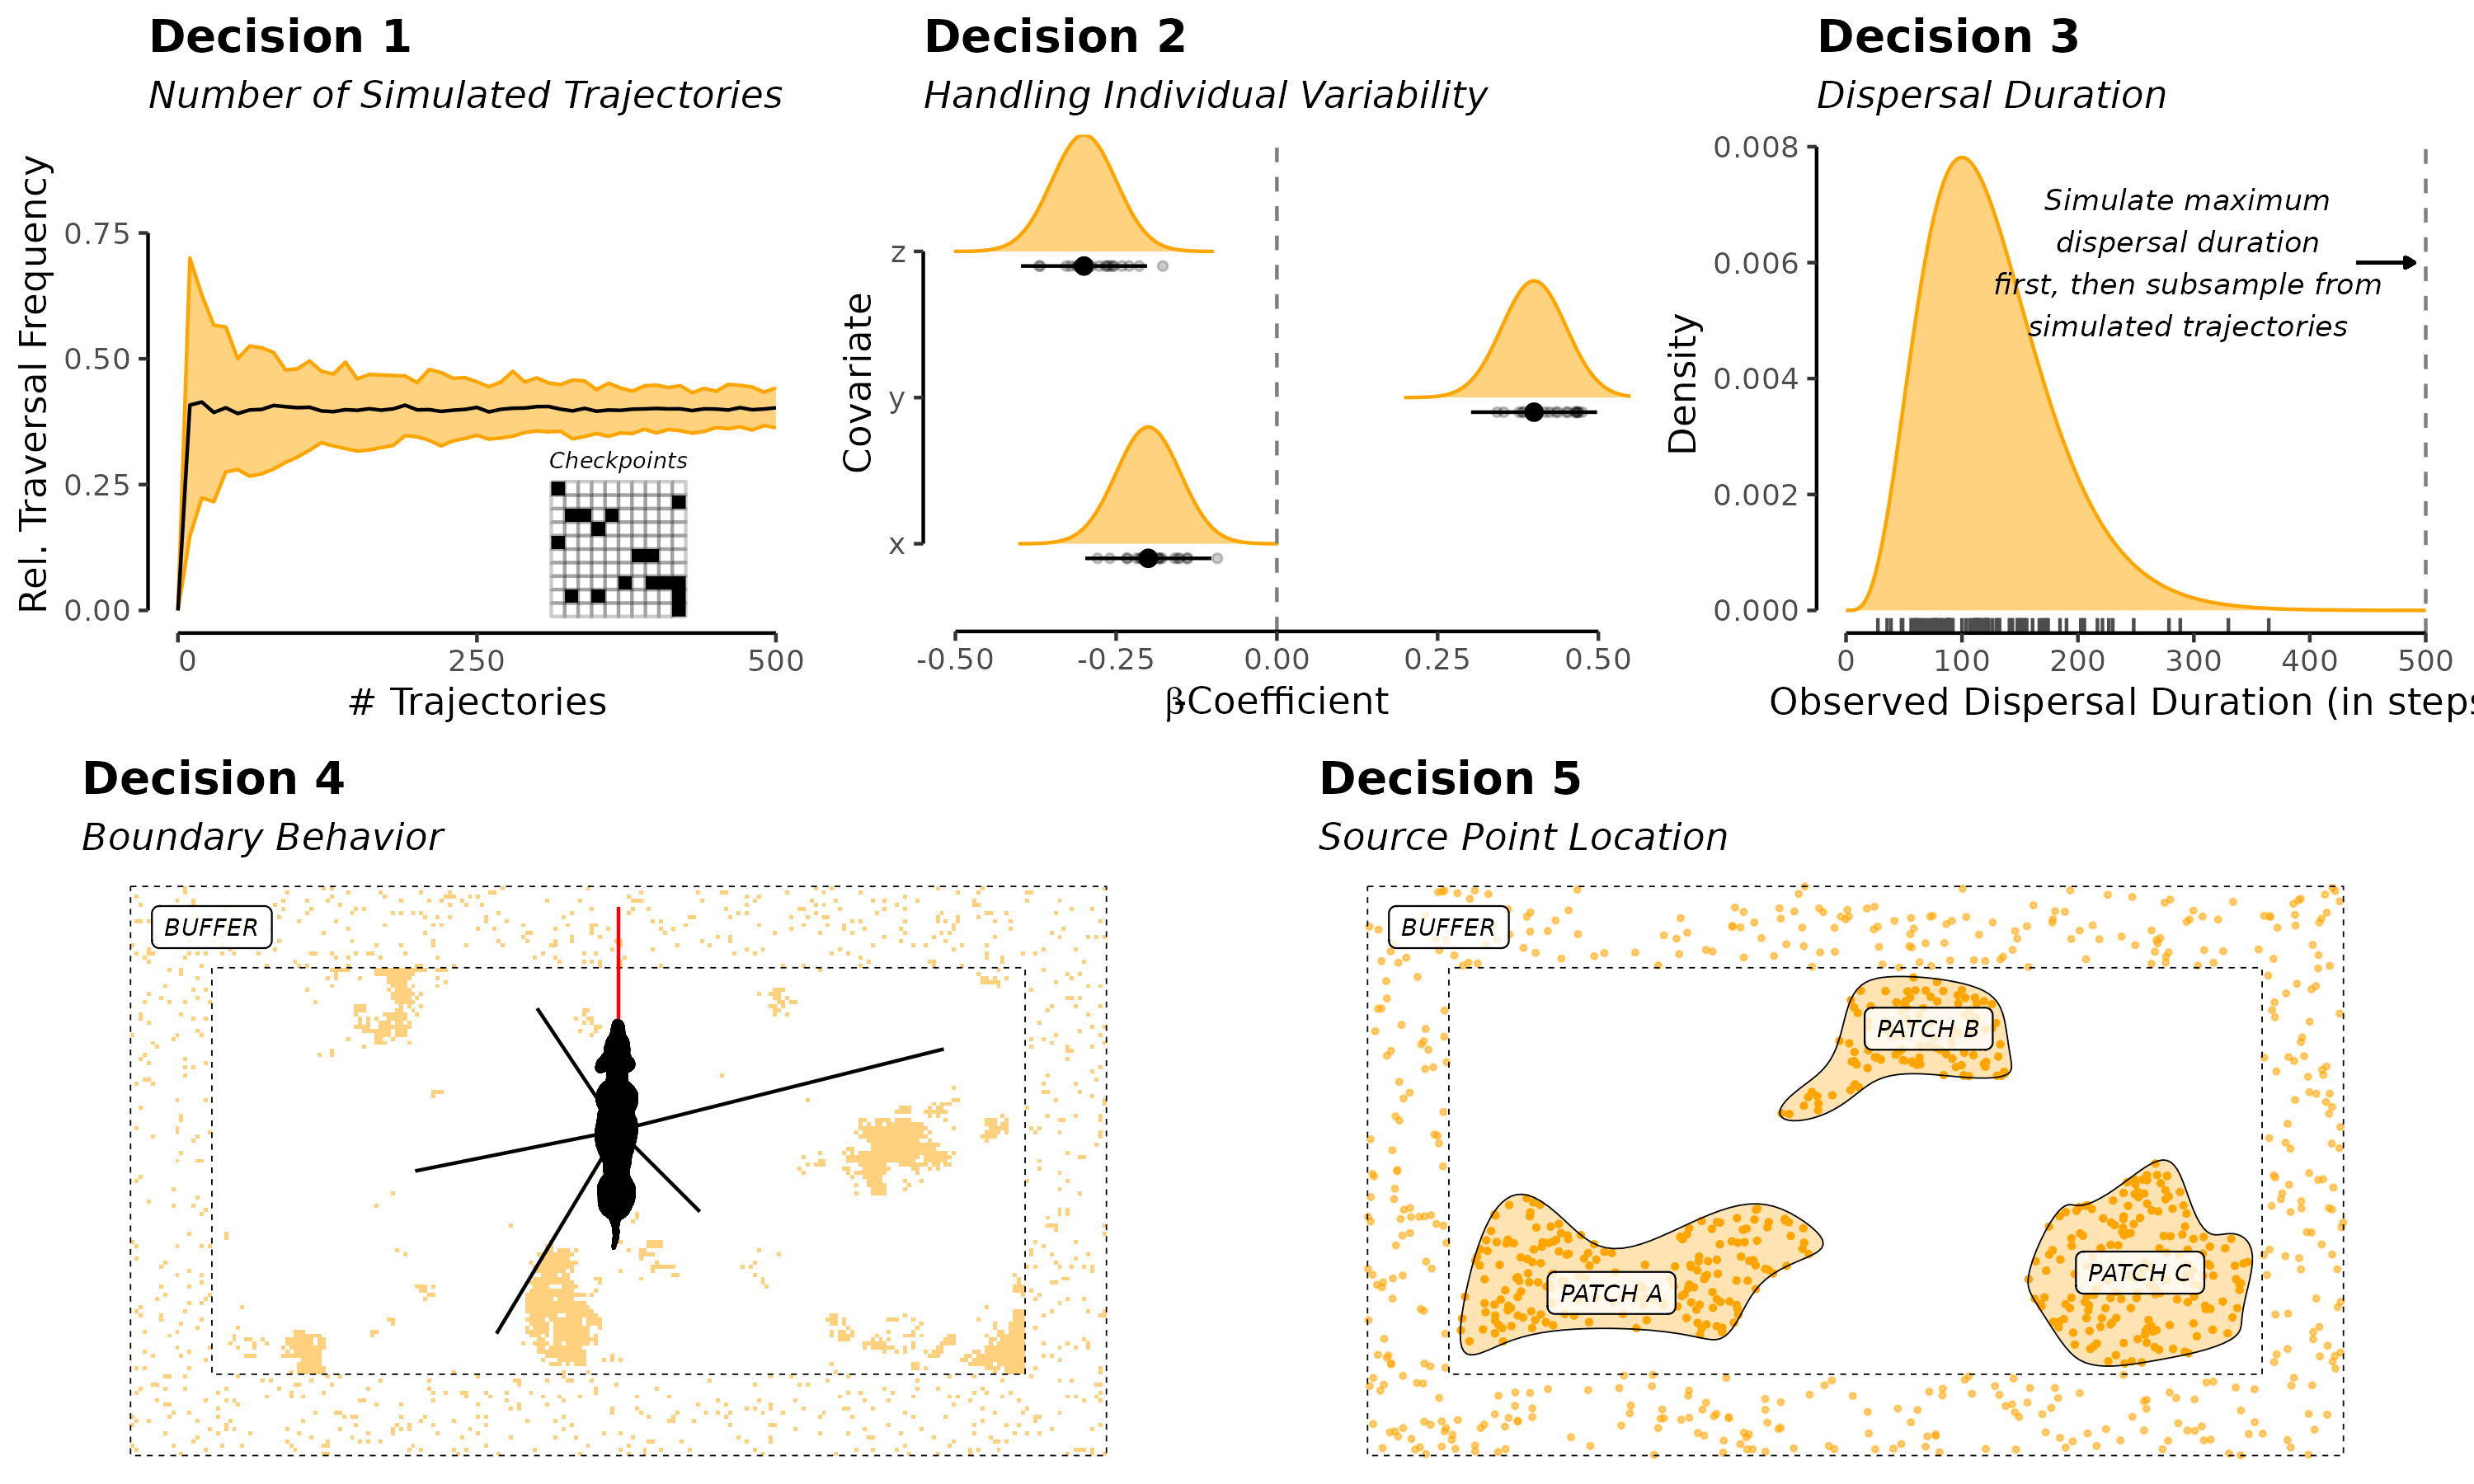
\includegraphics[width=\textwidth]{99_ModelingDecisions.png}
%   \caption{Five major modeling decisions that a researcher needs to consider
%   when simulating dispersers to assess landscape connectivity. (1) Number of
%   simulated trajectories. (2) Handling individual variation: we used point
%   estimates when simulating dispersers, assuming that there was no individual
%   variation. Alternatively, however, one could draw preferences for each
%   simulated individually based on model uncertainty. (3) Dispersal duration.
%   While one could draw the number of simulated steps based on observed dispersal
%   events, we opted for an alternative and simulated each individual for 2'000
%   steps, which was at the upper end of observed dispersal durations. This allows
%   to easily shorten the generated trajectories afterwards and to investigate the
%   sensitivity of results with regards to the dispersal duration. (4) Boundary
%   behavior. We allowed dispersers to leave and re-enter the main study area
%   through a buffer zone with randomized covariate values. Alternatively, one
%   could discard transgressing random steps, thereby forcing dispersers to remain
%   within the study area or simply terminate the simulation, assuming the
%   individual has disappeared. (5) Source point location. The location of source
%   points should optimally be biologically informed. For our simulation, we
%   placed source points within protected areas large enough to sustain viable
%   wild dog populations. Conceivable alternatives include placing source points
%   according to a habitat suitability model or based on abundance information.
%   Importantly, one must also consider potential immigrants from outside the main
%   study area.}
%   \label{ModelingDecisions}
% \end{figure}


\section{Authors' Contributions}
D.D.H., D.M.B., A.O. and G.C. conceived the study and designed methodology;
D.M.B., G.C., and J.W.M. collected the data; D.D.H. and D.M.B. analysed the
data; G.C. and A.O. assisted with modeling; D.D.H., D.M.B., and G.C. wrote the
first draft of the manuscript and all authors contributed to the drafts at
several stages and gave final approval for publication.

\section{Data Availability}
GPS movement data of dispersing wild dogs will be made available on dryad at the
time of publication. Access to R-scripts that exemplify the application of the
proposed framework to simulated data are provided through Github.

\section{Acknowledgements}
We thank the Ministry of Environment and Tourism of Botswana for granting
permission to conduct this research. We thank C. Botes, I. Clavadetscher, and G.
Camenisch for assisting with wild dog immobilizations. We also thank B. Abrahms
for sharing her data of three dispersing wild dogs. Furthermore, we are indebted
to Johannes Signer for assisting with the simulation algorithm. This study was
funded by Basler Stiftung für Biologische Forschung, Claraz Foundation, Idea
Wild, Jacot Foundation, National Geographic Society, Parrotia Stiftung, Stiftung
Temperatio, Wilderness Wildlife Trust Foundation, Forschungkredit der
Universität Zürich, and a Swiss National Science Foundation Grant
(31003A\_182286) to A. Ozgul.

\newpage
\begingroup
\singlespacing
\bibliography{Literatur}
\endgroup

\end{document}
